%\documentclass[12pt,a4paper,twoside]{book} 
\usepackage[spanish]{babel} % de pedro
\usepackage{graphics,graphicx,epsfig,color,float,afterpage,fancyheadings,subfigure,moreverb,alltt} % de pedro
\usepackage[latin1]{inputenc} % tildes de pedro

\usepackage{algorithm}
\usepackage{algorithmic}

\usepackage{rotating}
\usepackage{url}

%% Esta letra se convierte mejor a pdf que la normal
\usepackage{ae}

%%% Para las fuentes matemticas
\usepackage{amsfonts}

\usepackage{subfigure}

\usepackage{pstricks} % para los dibujos del da
\usepackage{lscape} % para las pginas en horizontal
\usepackage{portland} % para las pginas en horizontal
\usepackage{supertabular} % para las tablas de ms de una pgina
\usepackage{tabularx} % para las tablas del tipo tabularx
%\usepackage{glossary}
%\documentclass[a4paper,spanish,12pt]{book} % esto es de gustavo
%\usepackage{amsmath,amsfonts}   % underset mathbb
%\usepackage{authordate1-4}      % bib style
%\usepackage{epsfig}     % eps
\usepackage{epic}           % graficos
%\usepackage{eepic}           % graficos
\usepackage{curvesls}           % curvas
\usepackage{amssymb}
%\usepackage{fancyheadings}  % encabezados
%\usepackage{hhline}             % hhline
%\usepackage[latin1]{inputenc}   % tildes
%\usepackage{makeidx}        % ndices
%\usepackage{setspace}           % interlinea
%\usepackage[spanish]{babel} % espaol

%%%%%%%%%%%%%%%%%%%%%%%%%%%%%%%%%%%%%%%%%%%%%%%%%%%%%%%%%%%%%%%%%%%%%%%%%%%%%%%

\author{juanlu}
\title{Tesis de Juan Lus Jimnez Laredo}




\newcommand{\fecha}{\footnotesize{[ Impreso: \the\day-\ifcase\month\or
    Ene\or Feb\or Mar\or Abr\or May\or Jun\or Jul\or Ago\or Sep\or
      Oct\or Nov\or Dic\fi-\the\year ]}}

\newcommand{\N}{\mathbb{N}}

%% Para corregir las cabeceras largas
\newcommand{\cabecera}[2]{
\markright{\ref{#1}. \hspace{0.1ex} \MakeUppercase{#2}}}


%\pagestyle{headings}
%\renewcommand{\chaptermark}[1]{\markboth{\fecha \\ \\ #1}{}}
%\renewcommand{\sectionmark}[1]{\markright{#1 \\ \\ \fecha}}
%\addtolength{\headheight}{2.5pt}



%\lhead[\it\thechapter]{\sl\rightmark}
%\rhead[\rm\leftmark]{\it\thesection}
%\rfoot[]{\thepage}
%\cfoot[]{}
%\lfoot[\thepage]{}

%\thispagestyle{plain}

\setcounter{secnumdepth}{3}
\setcounter{tocdepth}{3}

%\renewcommand{\baselinestretch}{1.2}
%\setlength{\parskip}{0.8ex}

\newtheorem{theorem}{\sf Teorema}
\newtheorem{lemma}{\sf Lema}

\newcommand{\rem}[1]{\S\iffalse #1 \fi}
\newcommand{\cur}[1]{ {\it #1\/} }
\newcommand{\crcl}[1]{#1\kern-9pt\raise1pt\hbox{$\bigcirc$}}
\newcommand{\evag}{{\sf EvAg}}
\newcommand{\evagp}{{\sf EvAg.}}
\newcommand{\evags}{{\sf EvAgs}}
\newcommand{\evagsp}{{\sf EvAgs.}}

\newcommand{\prog}[2] {
   \small
   \begin{minipage}[t]{75mm} {\tt #1}  \end{minipage}
   \begin{minipage}[t]{60mm} {#2}      \end{minipage}
   \\
}
\newcommand{\prg}[2] { {\tt #1} & {\sf #2} \\}

\newcommand{\wmfspecial}[4]{
   \begin{figure}[h]
   \centerline{\psfig{figure=#1,height=#2}}
   \caption{#3}   \label{#4}
   \end{figure}
}                   % USO: \wmfspecial{nombre.eps}{altura}{leyenda}{etiqueta}

\def\stackunder#1#2{\mathrel{\mathop{#2}\limits_{#1}}}

\def\marco #1#2#3#4{\centerline{       % USO: \marco{.1}{10}{124mm}
  \vbox{\hrule height #1pt%
  \hbox{\vrule width #1pt\kern #2pt%
  \vbox{\kern #2pt%
  \vbox{\hsize #3\noindent #4}%
  \kern #2pt}%
  \kern #2pt\vrule width #1pt}%
  \hrule height0pt depth #1pt}} }


\newcommand{\symnote}[2]{\symbolnote{#1}{#2}}

\newfont{\bi}{cmbxti10 scaled\magstep1}       % bf + it


%% Ruta de las figuras
\graphicspath{{../figuras/}}


\begin{document}
           % Eliminarlo al compilar el documento maestro, ponerlo para compilarlo separado

%%%%%%%%%%%%%%%%%%%%%%%%%%%%%%%%%%%%%%%%%%%%%%%%%%%%%%%%%%%%%%%%%%%%%%%%%%%%%%%
%%                                                                           %%
%%                             Tesis Doctoral:                               %%
%%                        Juan Luis Jimenez Laredo                           %%
%%                                                                           %%
%%%%%%%%%%%%%%%%%%%%%%%%%%%%%%%%%%%%%%%%%%%%%%%%%%%%%%%%%%%%%%%%%%%%%%%%%%%%%%%


\cabecera{cap:evagperformance} {Experimental Analysis}%Descomentarlo para compilar maestro
\chapter{\textit{Experimental Analysis}}
\label{cap:evagperformance}
\cabecera{cap:evagperformance}{Experimental Analysis}%Descomentarlo para compilar maestro

%%%%%%%%%%%%%%%%%%%%%%%%%%%%%%%%%%%%%%%%%%%%%%%%%%%%%%%%%%%%%%%%%%%%%%%%%%%%%%%

In the previous chapter we have presented the \evag model as the framework in
which this thesis will analyse the viability of the P2P EC paradigm. In
addition, a first insight on the {\em computational performance} of the
approach has been provided showing that, for very demanding problems, it is able to scale holding linear speed-ups. 

Nevertheless, such results do not take into account whether the
  algorithm is able to converge to good solutions in spite of the
  run-time dynamics of P2P systems. Hence,  in this chapter, we propose 
%El capítulo no propone nada, lo haces tú - JJ
the experimental analysis of the model in a simulated P2P environment so that the viability of the P2P EA can be drawn from the {\em algorithmic performance} of the approach. All the source code for the experiments has been published under a GPL v3 license and is available from our Subversion repository at \url{https://forja.rediris.es/svn/geneura/evogen}.
  % Es suficientemente
  % importante como para que no lo relegues a una nota 

Simulations will allow the execution of controlled experiments tackling
the goals described in Section \ref{sec:goals} in which  a set of representative test-cases are proposed for
studying the viability of the model. In order to define the system with
a good level of detail, Section \ref{sec:decisions} describes the
decision-making process that we have followed for the experimental
analysis. Taking into account such decisions, Section
\ref{sec:overallmethodology} presents the overall methodology that will
be followed in the test-case 1 (Section \ref{sec:testcase1}), test-case 2 (Section \ref{sec:testcase2}) and test-case 3 (Section \ref{sec:testcase3}). Finally, conclusions on the {\em scalability} and {\em fault tolerance} of the model are drawn in Section \ref{sec:cap5:conclusions} based on the analysis of results.


 
%%%%%%%%%%%%%%%%%%%%%%%%%%%%%%%%%%%%%%%%%%%%%%%%%%%%%%%%%%%%%
\section{Goals}
\label{sec:goals}
%%%%%%%%%%%%%%%%%%%%%%%%%%%%%%%%%%%%%%%%%%%%%%%%%%%%%%%%%%%%%

As exposed at the \href{cap:introduccion}{introduction} of this thesis, one of the main motivations behind P2P EAs is tackling those large problem instances in which, due to memory or computational constraints, sequential approaches are unsuitable. In this sense, analysing the scalability of the \evag model is key to determine the viability of the approach. Additionally,
as the sizes of the problem instances increase, the number of computing nodes required to tackle the problem scales and, therefore, failures become more likely at run-time. Taking that into account, we propose an experimental analysis focusing on the following goals in order to prove the viability of the model:

\begin{enumerate}
\item Analysing the {\em scalability} of the model to demonstrate that the approach is suitable for tackling large problem instances in a failure-free environment.
\item Studying the {\em fault-tolerance} of the model under churn conditions to demonstrate that the model follows a {\em graceful degradation} and is able to tackle large problem instances in spite of nodes departing from the system.
\end{enumerate}


Studying the scalability makes possible not only  to analyse instances
under examination  % He cambiado esta frase, pero sigo sin
		   % entencerla. Será instance sizes?
		   % Modificada la continuacion de la frase- Juanlu
but also predicting the model behaviour when tackling larger instances. On the other hand,  fault tolerance is a key issue in a P2P EA since churn is inherent to P2P systems given that peers are prone to failures.  


In order to tackle such goals, the following test-cases have been designed to assess the algorithm performance:

\begin{enumerate}
\item {\em Scalability of the model in failure-free environments against sequential approaches}. The \evag model is compared against a canonical SSGA and a GGA to demonstrate that such a spatially-structured EA scales better than panmictic schemes of evolution.

\item {\em Influence of the population structure on the algorithm performance}. As explained in Section \ref{sec:evag}, there is no reason preventing the \evag model to use population structures other than newscast. Therefore, this test-case aims analysing the scalability of the model using two common topologies in fine-grained approaches: a ring lattice \cite{giacobini:regular} and a Watts-Strogatz \cite{giacobini:evocop06} population structures.

\item {\em Fault tolerance of the model}. In this test-case, we will analyse the scalability of the model using several scenarios of churn in which the system degrades under different failure rates.
\end{enumerate}

Before proceeding with the experimental analysis, the following section describes all the decisions related with the implementation of the model.



%%%%%%%%%%%%%%%%%%%%%%%%%%%%%%%%%%%%%%%%%%%%%%%%%%%%%%%%%%%%%
\section{Rationale for the experimental analysis}
\label{sec:decisions}
%%%%%%%%%%%%%%%%%%%%%%%%%%%%%%%%%%%%%%%%%%%%%%%%%%%%%%%%%%%%%

Given the huge complexity of either P2P systems or EAs, a detailed
analysis on their interactions in the P2P EC paradigm remains  % o lays
				% - JJ
 beyond the scope of this thesis. Hence, a certain number of decisions has to be made in order to focus the analysis on the specifications of the goals. Therefore, this section aims to justify the simplifications and assumptions made on the model.


\subsection{Simplifications}

In order to simplify the analysis on the model performance, the following considerations were made on the design of experiments:
% No tengas comienzos vacíos. Por ejemplo, la última frase de la
% introducción podías ponerla aquí - JJ


\begin{itemize}
   \item The experimental analysis in this thesis will concentrate on {\em binary-coded GAs} \cite{michalewicz:ga}, excluding the rest of EC paradigms such as ES \cite{es:rechenberg}, EP \cite{ep:fogel} or GP \cite{gp:koza}. The main reason for this restriction is that the population sizing theory \cite{goldberg:competent} that we will follow to perform analysis on the scalability of the algorithm focuses on such a kind of EAs.  Nevertheless, taking into account that {\em binary-coded GAs} follow the same evolutionary scheme than other EAs such as {\em real-coded GAs} \cite{rcga:eshelman} or GP, conclusions should be easily extended to other paradigms.
   
   \item With the aim of establishing a worst-case analysis,
	 evolutionary operators will not apply specific knowledge on the
	 problem. In this context, we will use  {\em uniform crossover} and
	 {\em bit-flip mutation} as variation operators and {\em binary
	 tournament} as decentralised selection mechanism throughout all
	 the experiments \cite{eiben:eas}. 
    Taking into account that we will use trap functions as benchmark (described in Section \ref{sec:benchmark}), either {\em uniform crossover} or {\em bit-flip mutation} prevent the algorithm
	 search to form higher order BBs, thus challenging the GA's search mechanisms. On an averaged sense, such operators are fooled by traps as described by Deb and Goldberg in \cite{deb:deception}.
     % esto no acabo de creérmelo, así que
	 % tendrías que justificarlo. Los higher-order BBs pueden
	 % crearse por selección, y si los mendas son muy parecidos, se
	 % preservan con el uxover - JJ
	 % - Cierto, es algo que no se cumple en general, pero si que ocurre en funciones trampa. Añado comentario a las traps y referencia a Deb. - Juanlu

   \item In the same line of the previous point, individuals will be {\em initialised at random}. Every gene will have an uniform probability of $0.5$ of being either $1$ or $0$, so that, on average, the randomly generated initial population is placed on local optimum attracting regions for the problem landscapes proposed in Section \ref{sec:benchmark}.
   
\end{itemize}

\subsection{Assumptions}

The experimental analysis in this chapter examines the main variables influencing the \evag performance. To that aim, experiments were designed in such a way that variables under study can be analysed by assuming fixed conditions for the rest of factors. Such assumptions are detailed in the following points:

% Igual aquí. Mete algo.  - JJ

\begin{itemize}
   
   \item We have used selectorecombinative versions of the algorithms
	 (without mutation) for estimating the population sizes. Lobo
	 and Lima state in \cite{lobo07:review} that the assumption of a
	 selectorecombinative GA is commonly made in population sizing
	 studies. That way, the only source of diversity is then the initial
	 population which stands for a worst case analysis. However,
	 this thesis complements the study analysing the convergence of
	 the approach using mutation. 
   
    \item We assume that every \evag behaves as a {\em virtual node}
	  \cite{dynamo:virtualnodes} in such a way that every physical
	  node can host more than a single \evagp Hence, the number of
	  {\em virtual nodes} hosted in a physical one can be decided at
	  a load-balancing level depending on node capacities and a
	  heterogeneous system such as P2P can be assumed as homogeneous
	  at a virtual level. 
   
   \item Despite having assumed homogeneous conditions in the previous
	 point, the lack of a central clock in a decentralised scheme
	 implies an asynchronous execution. In this sense, the most
	 commonly used methods to simulate asynchrony either in cellular
	 automaton \cite{asynchrony:ca} or cellular evolutionary
	 algorithms \cite{tomassini} can not be applied in this case except for the {\em Uniform choice} policy, more appropriate to model a decentralised run in which there is no guarantee of any sequential order in the update of the individuals. In Uniform choice, the next agent to be updated is randomly chosen with uniform probability from all the possible cells. This method implies that the same agent could be updated more than once during a cycle and, in turn, some others could remain without updating.  This way, we have adopted such a policy to simulate the asynchronous update of \evagsp
   
%  \begin{itemize}
%   \item {\em Fixed line sweep}, the idea here is that the update on the different cells (i.e. \evag in our case) follows a prestablished sequential order, e.g. from left to right in rings structured populations.
%   \item {\em Fixed random sweep}, it consists in a small variation on the previous method in which the update sequence is set randomly at the beginning of a run as a permutation of the different cells.
%   \item {\em New random sweep}, a new random cell permutation is generated at every cycle of a run, understanding a cycle (or time step) as the sequential update of all the cells. 
%   \item {\em Uniform choice}, the next cell to be updated is randomly chosen with uniform probability from all the possible cells. This method implies that the same cell could be updated more than once during a cycle and, in turn, some others could remain without updating.
%   \end{itemize}
   
% No me parece que lo de arriba venga muy a cuento. Sería mejor que
	 % dijeras que has elegido uniform, y que hay otros tipos que no
	 % te vienen bien porque requieren una secuencia. La morralla,
	 % cuando menos mejor - JJ 
% Yo creo que es interesante ponerlo, por un lado no ocupa mucho y por otro, son las cuatro tecnicas que se suelen utilizar, si se explican las cuatro es mas facil justificar el hecho de porque se ha elegido la que se ha elegido. - Juanlu
%To the choice of an adequate update policy for our approach,  the {\em uniform choice} policy seems more appropriate to model a decentralised run in which there is no guarantee of any sequential order in the update of the individuals. This way, we have adopted such a policy to simulate the asynchronous update of \evagsp

%In addition, it has to be considered that Dorronsoro et al. show in
%	 \cite{dorronsoro:asynchrony} that the four methods do not
%	 always %always? - JJ
% present statistical differences between each other in a test-suite of four
	 % no uses números en el texto, usa la palabra. - JJ
% different problems. The uniform choice method presents statistical
%	 differences from the rest in a single case, indicating that
%	 choosing between these methods does not have a great influence
%	 on the algorithm performance. 

   \item With respect to the update frecuency of an \evag, it has to be consider that there are two independent tasks running in parallel within every agent, the evolutionary loop and the newscast protocol. In this sense, we have assumed that every time an \evag performs a fitness evaluation, it also initiates a cache exchange of the
	 newscast protocol, i.e. $t_r=cycle$ where $t_r$ is the
	 parameter for the newscast updating frequency exposed in
	 Section \ref{sec:p2pnewscast} and {\em cycle} is defined as the
	 time the algorithm takes to perform $n$ evaluations in a
	 population of $n$ \evags using {\em uniform choice}.
   
   \item As it has already been shown in Section \ref{sec:bootstrapping}, the newscast protocol takes at around 12 cycles to converge to an state of dynamic equilibrium for a network size of $1600$ which is the maximum size that we have used here. In this sense, the evolutionary algorithm  will begin at $t_r=20$ in order to guarantee that the  protocol bootstraps and converges. We have assumed a synchronised start up of the experiments. 

  \item The cache size ($c$) is the only tunable parameter in newscast and we use $c=20$ within all the settings of the experiments. Such value takes into account Jelasity and van Steen recommendations in \cite{jelasity:newscast} stating that the intended normal setting of newscast is $c \ll n$ and demonstrating that values from $c=20$ prevent the spontaneous partitioning of the graph even when it becomes very large (see Section \ref{sec:newscastrobustness} for more details). In addition, we make experiments for the fine-tuning of the parameter in the appendix \ref{cap:appendixA} of this thesis showing a lack of influence of $c$ on the \evag performance when $c \in [0.01n,0.16n]$, where $n$ is the population size.

 \item We have assumed that the time required for communications is
       negligible with respect to the fitness computing time. Such an assumption might be unrealistic for
       small problem instances, but it turns feasible for problem instances
       becoming large. As it has been shown in the analysis of the
       parallel performance of the model in Section \ref{sec:parallelperformance}, communications do not inflict a penalisation on the algorithm speed-up for problems with a very demanding fitness evaluation cost.
       
       % How large? A partir de cuánto
       % no tiene importancia? Esto no creo que sea cierto, pero
       % bueno... tienes que justificarlo mejor - JJ
       % He añadido una ultima frase haciendo referencia a los resultados previos en escalabilidad. Cuando una instancia es suficientemente costosa, el tiempo de comunicacion es despreciable con respecto al de comunicacion. - Juanlu

 
\end{itemize}

% Ninguna conclusión o sumario - JJ

Once assumptions have been laid out, we will continue describing the experimental methodology next.




%%%%%%%%%%%%%%%%%%%%%%%%%%%%%%%%%%%%%%%%%%%%%%%%%%%%%%%%%%%%%
\section{Experimental Methodology}
\label{sec:overallmethodology}
%%%%%%%%%%%%%%%%%%%%%%%%%%%%%%%%%%%%%%%%%%%%%%%%%%%%%%%%%%%%%

%This thesis analyses the scalability of the \evag model from the perspective of the population sizing theory \cite{gwoldberg:competent}  which states that there is an optimal criterion for tuning the population size of an EA for a given problem instance and difficulty. Within this thesis, the population size has been empirically estimated using the method explained in Section \ref{sec:bisection} that tunes the minimum population size $N$ required to supply enough building blocks (BBs) so that a selectorecombinative Genetic Algorithm (GA) will converge toward optimal solutions. The assumption of a selectorecombinative GA (without mutation) is commonly made in population sizing studies as the only source of diversity is then the initial supply of raw BBs which stands for a worst case analysis \cite{lobo07:review}.


In order to analyse the scalability of the \evag model, experiments are
conducted on trap functions (described in Section
\ref{sec:benchmark}). %Incluye hyperref, creo, para que genere
		      %hiperenlaces internos automáticamente
 The purpose is investigating how population sizes scale with increasing problem size and difficulty. To this end, we follow the population sizing theory \cite{goldberg:competent} which states that there is an optimal population size for a given problem instance that can be determined under some conditions. In particular, we use the bisection method (which will be explained in Section \ref{sec:bisection}) that determines the minimum population size $N$ for a selectorecombinative GA. 
%The assumption of a selectorecombinative GA is commonly made in population sizing studies as the only source of diversity is then the initial population which stands for a worst case analysis \cite{lobo07:review}. 
In addition, we look at the scale-up properties of the average number of evaluations to a solution (AES), which is an algorithmic independent measure of computational effort that can be used for all EAs, with or without mutation \cite{eiben:eas}. Finally, the study is complemented switching mutation on, so that the algorithm convergence is analysed for the most demanding problem instances using the metrics that will be proposed in Section \ref{sec:metrics}. Such results will be statistically analysed using the non-parametric Wilcoxon test \cite{salva09:wilcoxon}  within the following Sections.




\subsection{Test-suite for the experiments}
\label{sec:benchmark}
%%%%%%%%%%%%%%%%%%%%%%%%%%%%%%%%%%%%%%%%%%%%%%%%%%%%%%%%%%%%%

%No está bien comenzar con un gerundio, porque necesitas varias líneas
%para saber qué es lo qeu estás haciendo siguiendo a Lobo y Lima. Di que
%haces, y luego por qué - JJ
% Modificado! - Juanlu
Experiments were conducted on deceptive, quasi-deceptive, and non-deceptive trap functions \cite{ackley:trap}
following Lobo and Lima's recommendations in \cite{lobo07:review} about choosing a test suite with known population requirements and investigating the scalability on landscapes with different characteristics.  These functions represent a set of decomposable problems based on unitation and composed of sub-functions in which the total fitness is additively calculated by summing the partial fitness of every sub-function. Hence, it is easy to scale the problem from small to large instances by considering a smaller or larger number of sub-functions. In addition, each sub-function is composed of ($k$) bits representing the BB size, every sub-function is then composed of $2^k$ combinations from which only one belongs to the optimal solution. Considered values include $k=2$, $k=3$ and $k=4$ (forming non-deceptive, quasi-deceptive and deceptive problems respectively). Studying the scalability for different settings of $k$ can offer a better understanding of the model since not only the scalability is analysed but also how the scalability changes as the problem difficulty increases. 

%No queda bien empezar con una preposición una frase. Comienza con el
%sujeto: there are two...
There are two distinct regions in the search space of trap functions, one leading to a global optimum and the other leading to the local optimum (see Figure \ref{fig:trap}).  In general, a trap function is defined by the following equation:


\begin{equation} \label{eq:trap}
trap(u(\overrightarrow{x}))=\left\{
\begin{array}{ll}
\frac{a}{z}(z-u(\overrightarrow{x})), & \mbox{if}\quad u(\overrightarrow{x}) \leq z \\
\frac{b}{l-z}(u(\overrightarrow{x})-z), & \mbox{otherwise}
\end{array} \right.
\end{equation}

\noindent
where $u(\overrightarrow{x})$ is the unitation function, \textit{a}\ is the local optimum, \textit{b}\ is the global optimum, \textit{l}\ is the problem size and \textit{z}\ is a slope-change location separating the attraction basin of the two optima. 

%%%%%%%%%%%%%%%%%%%%%%%%%%%%%%%%%%%
\begin{figure}[!htpb]
\centerline{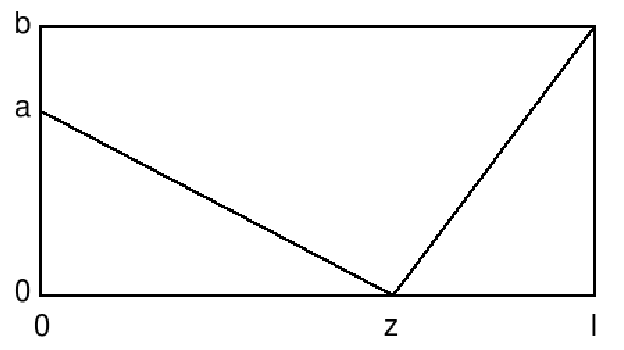
\includegraphics[width=2in]{trap}}
% este gráfico es cutre, se nota que es un jpg convertido. ¿No se puede
 % hacer mejor? - JJ
\caption{Generalised \emph{l-trap} function. }
\label{fig:trap}
\end{figure}
%%%%%%%%%%%%%%%%%%%%%%%%%%%%%%%%%%%


For the following experiments, 2-trap, 3-trap and 4-trap functions were designed with the following parameter values: $a = l-1$, $b = l$, and $z = l-1$. With these settings\footnote{Originally, Ackley's trap functions use $z=\frac{3l}{4}$, however, Deb and Goldberg demonstrate in \cite{deb:deception} that trap functions are fully easy under such settings.}, 2-trap  is not deceptive, 4-trap is deceptive and 3-trap lies in the region between deception and non-deception. Under these conditions, it is possible not only to examine the scalability on trap functions, but also to investigate how the scalability varies when changing from non-deceptive to deceptive search landscapes.
Scalability tests were performed by juxtaposing \textit{m}\ trap functions in binary strings of length $L$ and summing the fitness of each sub-function to obtain the total fitness. 


\subsection{A method for estimating the population size}
\label{sec:bisection}
%%%%%%%%%%%%%%%%%%%%%%%%%%%%%%%%%%%%%%%%%%%%%%%%%%%%%%%%%%%%%

Sastry proposes in \cite{sastry:bisection} a method based on bisection to  estimate
the optimal population size $N$ to solve a problem instance, that is, the lowest $N$ for which
98\% of the runs find the problem optimum. To this end, a selectorecombinative GA is used to search the minimum population size such that using random initialisation it is able to converge to the optimum without any other mechanism than recombination and selection. 

%%%%%%%%%%%%%%%%%%%%%%
\begin{algorithm}
\caption{Population tuning algorithm based on bisection}
\label{alg:bisection}
\begin{algorithmic}
\STATE $N$ = Initial Population Size ($20$)
\WHILE{ GA reliability ($N$) $<$ 98\%}
\STATE $min = N; max,N = 2N$
\ENDWHILE
\WHILE{ $\frac{max-min}{min} > \frac{1}{16}$}
\STATE $N = \frac{max+min}{2}$ 
\IF{ GA reliability($N$) $<$ 98\%}
\STATE $min = N$
\ELSE
\STATE $max = N$
\ENDIF
\ENDWHILE
\end{algorithmic}
\end{algorithm}
%%%%%%%%%%%%%%%%%%%%%%



Algorithm \ref{alg:bisection} depicts the method based on bisection.
The method begins with a small population size which is doubled until
the algorithm ensures a reliable convergence. After that, the
interval $(\mathit{min},\mathit{max})$ is halved several times and the population size
adjusted within such a range until $\frac{\mathit{max}-\mathit{min}}{\mathit{min}} > \mathit{threshold}$,
where $\mathit{min}$ and $\mathit{max}$ stand respectively for the minimum and maximum population size estimated and $\mathit{threshold}$ for the accuracy of the adjustment within such a range. This parameter has been set to $\frac{1}{16}$ in order to obtain a reasonable adjustment of the population size, e.g. the algorithm would estimate a population size of $N=310$ if we consider an optimal size of $N=315$.




\subsection{Metrics}
\label{sec:metrics}
%%%%%%%%%%%%%%%%%%%%%%%%%%%%%%%%%%%%%%%%%%%%%%%%%%%%%%%%%%%%%

The following metrics % Trata de cualificar siempre que
 % puedas las citas: as proposed by, as we have published in, as
 % reviewed by... tal como lo has puesto, no sé si es una descripción de
 % las métricas, una justificación de las mismas, o qué...
 % Si, quedaba raro. - Juanlu
 will be used for assessing the performance of the model in the experimental analysis. To allow the comparison of results with those in the literature such metrics were chosen to be standard in EAs. Either Tomassini in \cite{tomassini} or Eiben and Smith in \cite{eiben:eas} make an extensive revision of them.
 

\begin{itemize}
\item The success rate (SR) measures the algorithm quality as the proportion in which the algorithm is able to find the problem optimum out of all the runs. 

\item The average number of evaluations to solution (AES) stands for the
      number of evaluations that the algorithm spends in those runs that
      yield success. Since a preliminary analysis on the normality of
      results shows that they do not follow a normal distribution, we
      have chosen the number of evaluations to solution in the third
      quartile ($AESQ_3$) as a baseline value, meaning that
      75\% of the runs will stay below such a value. % Third no es muy
      % central. Quizás es indicativo, pero central ni de coña.. - JJ
      % Sustituido por Value of reference - Juanlu

\item The Mean Best Fitness (MBF) is used to depict the algorithm convergence as the averaged values of the best fitness.

\item The genotypic distance entropy (GE) is a measure of the population diversity
  defined on the genotypic distances ($H_g(P)$). 

\begin{equation}
H_g(P)=-\sum_{j=1}^{N}{g_jlog(g_j)}
\end{equation}

\noindent where $g_j$ is the fraction $\frac{n_j}{N}$ of individuals in $P$ having a Hamming distance $j$ to
a genotype of reference (we have used the optimal genotype to that end), and $N$ is the number of different distances.

\end{itemize}





%%%%%%%%%%%%%%%%%%%%%%%%%%%%%%%%%%%%%%%%%%%%%%%%%%%%%%%%%%%%%
\subsection{Summary}
\label{sec:methodolgyconclusions}
%%%%%%%%%%%%%%%%%%%%%%%%%%%%%%%%%%%%%%%%%%%%%%%%%%%%%%%%%%%%%

This section has presented the experimental methodology that will be followed for analysing the viability of the \evag approach. To that aim, we will have to prove that the algorithm is {\em scalable} and {\em fault-tolerant} in a simulated P2P environment.

In order to tackle such goals, we will perform an experimental analysis of the three test-cases summarised in Table \ref{table:methodology}. In every case, the analysis will follow the same methodology, consisting in the study of the algorithmic scalability, the analysis of the algorithm convergence and population diversity at run-time and a comparison of the results to show whether they present statistical differences or not.


\begin{sidewaystable}[htbp]
%\begin{table}[htbp]
\centering
{\small
\begin{tabular}{|c | c|}
\hline
Test-Case & Methodology \\
\hline
1 & 1.1 Scalability selectorecombinative GA\\
Scalability in a failure-free environment & 1.2 Analysis of the convergence of the larger problem instance\\
vs. sequential GAs& 1.3 Statistical analysis\\
\hline
2 & 2.1 Scalability selectorecombinative GA\\
Influence of the population structure & 2.2 Analysis of the convergence of the larger problem instance\\
on the algorithm performance & 2.3 Statistical analysis\\
\hline
3 & 3.1 Scalability selectorecombinative GA \\
Fault tolerance of the model & 3.2 Analysis of the convergence under different churn scenarios\\
& 3.3 Statistical analysis\\
\hline
\end{tabular}
}
\caption{Summary of the experimental methodology.\label{table:methodology}}
%\end{table}
\end{sidewaystable}



\clearpage
%%%%%%%%%%%%%%%%%%%%%%%%%%%%%%%%%%%%%%%%%%%%%%%%%%%%%%%%%%%%%
\section{Test-Case 1: Scalability of the model in failure-free environments}
\label{sec:testcase1}
%%%%%%%%%%%%%%%%%%%%%%%%%%%%%%%%%%%%%%%%%%%%%%%%%%%%%%%%%%%%%



%Within this context, Peer-to-Peer (P2P) systems provide a powerful parallel infrastructure able to constitute a single virtual computer composed of a potentially large number of interconnected resources \cite{wehrle05:p2p}. Such a computing paradigm defines a rich set of topologies for the interconnection of nodes at application level, so-called overlay networks. Hence, a distributed P2P EA can be designed as an EA in which the population structure is defined by a P2P overlay network \cite{upali:adaptive}. That is, any given individual has a restricted number of neighbours and the chances for mating are, therefore, restricted to the P2P neighbourhood. 

%Interactions in such a spatially structured EA can be visualized as a graph. As shown in \cite{tomassini}, vertices represent individuals and edges the relationships between them. In this sense, the sequential approach is represented as a complete graph by default (alternatively called panmictic graph) whereas parallel approaches define a richer set of graph structures such as regular lattices \cite{giacobini:regular}, toroid \cite{giacobini:gecco04} or small-world \cite{giacobini:gecco05}, \cite{preuss04ppsn}, \cite{giacobini:evocop06}. Based on these studies, the Evolvable Agent model (\evag) presented in \cite{laredo:cec2008} is a distributed and decentralized P2P EA in which the population structure of the EA is defined by a gossiping protocol called newscast that behaves asymptotically as a small-world graph \cite{jelasity:gossip}, \cite{jelasity:newscast}. This way, the \evag model is designed to be massively parallel in order to reduce the execution time of the algorithm while preserving the quality of the solutions. 


In order to investigate the scalability of the \evag model, experiments were conducted on different trap functions and compared against two canonical GAs, a steady-state GA (SSGA) and a generational GA (GGA).   Whereas the population structure of the \evag model is defined by the newscast protocol, the canonical GAs are panmictic. 
Following the experimental methodology of Section \ref{sec:overallmethodology}, two series of experiments were conducted:

In the first series that will be presented in Section \ref{cap5:testcase1:sca}, experiments use selectorecombinative versions of the GAs to estimate optimal population sizes for the different problem instances. The reason for using selectorecombinative GAs is that there are well defined models to establish the population size and the number of evaluations required to solve a given trap function instance \cite{harik:gambler}, however, to the best of our knowledge there are no such models when using mutation. To this end, in Section \ref{sec:bisection} we have described a method for estimating the population size. 
The underlying idea is that without mutation, the population size becomes the only source of diversity. 
In this context, Thierens demonstrates in \cite{thierens:scalability} the necessity of larger population sizes when tackling larger problem instances.

In the second series presented in Section \ref{cap5:testcase1:conver}, the analysis focuses on the performance of the different approaches when they are equally parametrised. Specifically, large instances of 2-Trap, 3-Trap and 4-Trap are considered to analyse the convergence of the fitness and the evolution of genotypic diversity. Finally, such results are statistically analysed in order to determine whether the difference in performances are significant or not.

\subsection{Scalability analysis}
\label{cap5:testcase1:sca}
%%%%%%%%%%%%%%%%%%%%%%%%%%%%%%%%%%%%%%%%%%%%%%%%%%%%%%%%

In this first series of experiments, different approaches have no mutation in order to
meet the selectorecombinative criterion of the bisection method. All settings are summarised in Table \ref{table:testcase1_sca_parameters} taking into account decisions in Section \ref{sec:decisions} about choosing operators that do not take advantage of the problem structure or setting the cache size. Since the methodology imposes a SR of 0.98 in the results, the $AESQ_3$ has been
used as an appropriate metric to measure the computational effort to reach the success criterion. A more efficient algorithm will need a
smaller number of evaluations.

%%%%%%%%%%%%%%%%%%%%%%%%%%%%%%%%%%%%%%%%%%%%%%%%%%%%%%%%
\begin{table}[htbp]
\centering
{\scriptsize
\begin{tabular}{r l}
\multicolumn{2}{l}{\textbf{Trap instances}}\\
\hline
BB size & $2, 3, 4$\\
Individual Length ($L$) & $12, 24, 36, 48, 60$\\
&\\
\multicolumn{2}{l}{\textbf{GA settings}}\\
\hline
GA & selectorecombinative SSGA \\
& selectorecombinative GGA\\
& selectorecombinative \evag \\
Population size & Tuning algorithm\\
Selection of Parents & Binary Tournament\\
Recombination & Uniform crossover, $p_c = 1.0$ \\
&\\
\multicolumn{2}{l}{\textbf{Newscast settings}}\\
\hline
Cache size & 20\\

\end{tabular}
}
\caption{Test-case 1: Parameters of the experiments in the analysis of scalability. \label{table:testcase1_sca_parameters}}
\end{table}
%%%%%%%%%%%%%%%%%%%%%%%%%%%%%%%%%%%%%%%%%%%%%%%%%%%%%%%%




Figure \ref{fig:popq3es} depicts the scalability of the population size ($N$) and the required number of evaluations to reach the problem optimum ($AESQ_3$) for the three approaches under study on
2, 3, and 4-trap functions. All the graphics show that either the population size or the computational effort fit with a potential order of scalability with base the length of the chromosome ($L$) and different exponents depending on the problem difficulty and the approach itself. 



%%%%%%%%%%%%%%%%%%%%%%%%%%%%%%%
\begin{figure*}[!htpb]
\centering
\centering
\subfigure{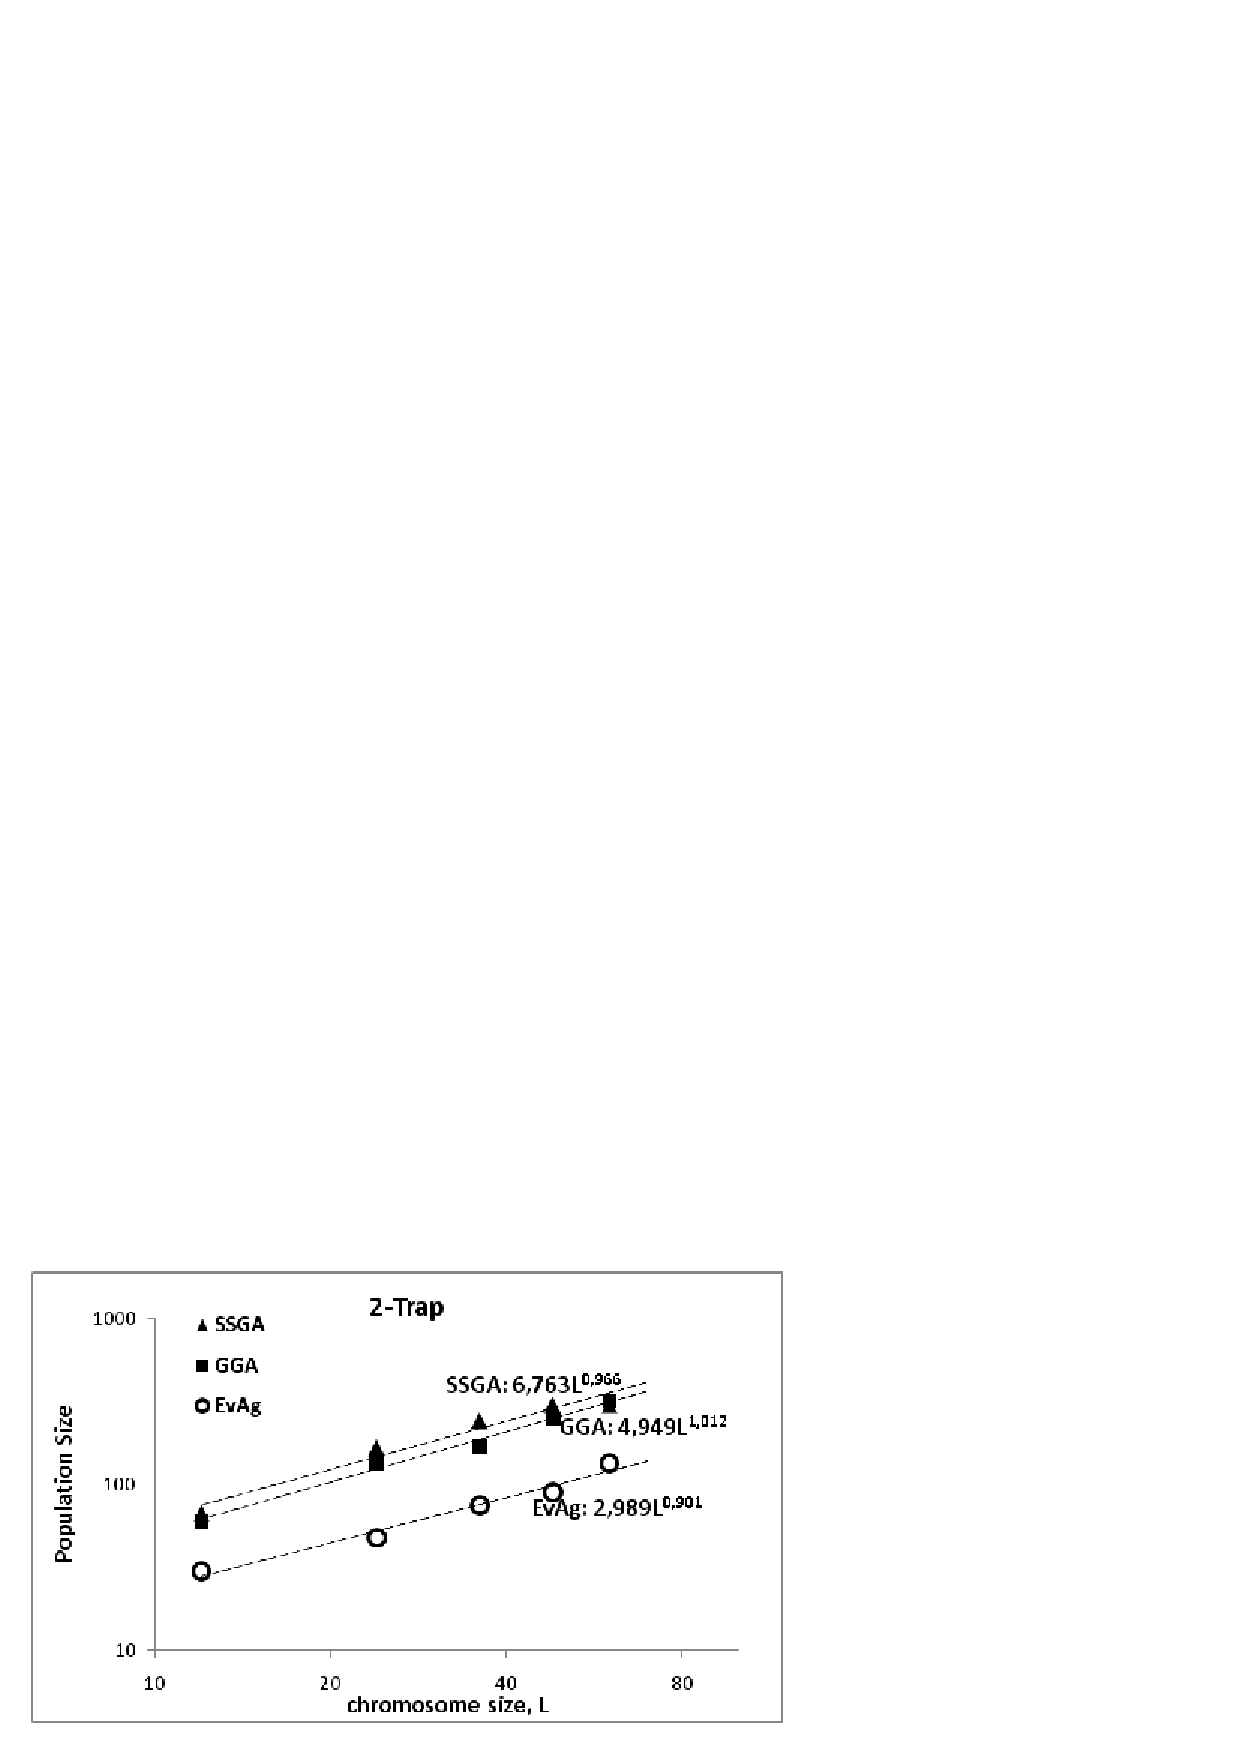
\includegraphics[width=2.9in]{2trappop}}
\hspace{1pt}
\subfigure{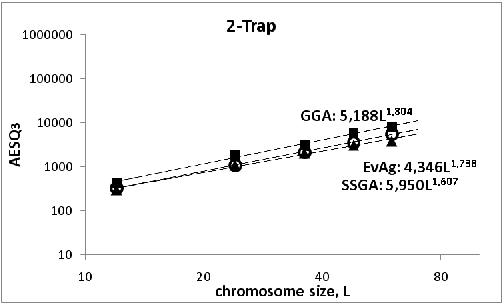
\includegraphics[width=2.9in]{2trapq3es}} \\
\subfigure{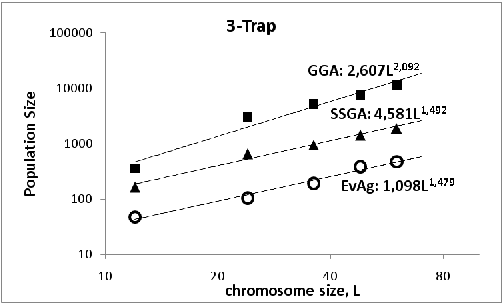
\includegraphics[width=2.9in]{3trappop}}
\hspace{1pt}
\subfigure{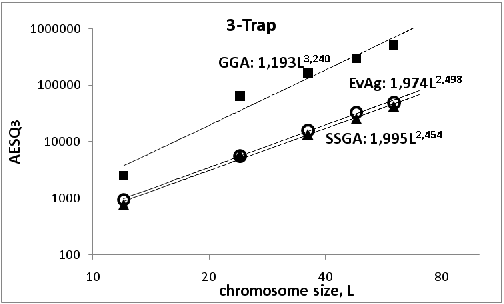
\includegraphics[width=2.9in]{3trapq3es}}\\
\subfigure{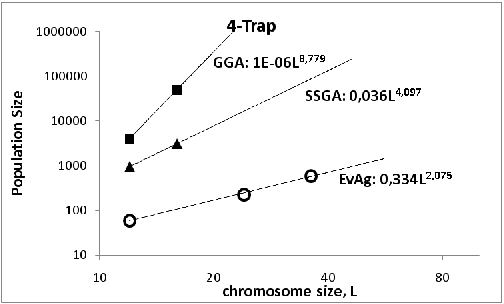
\includegraphics[width=2.9in]{4trappop}}
\hspace{1pt}
\subfigure{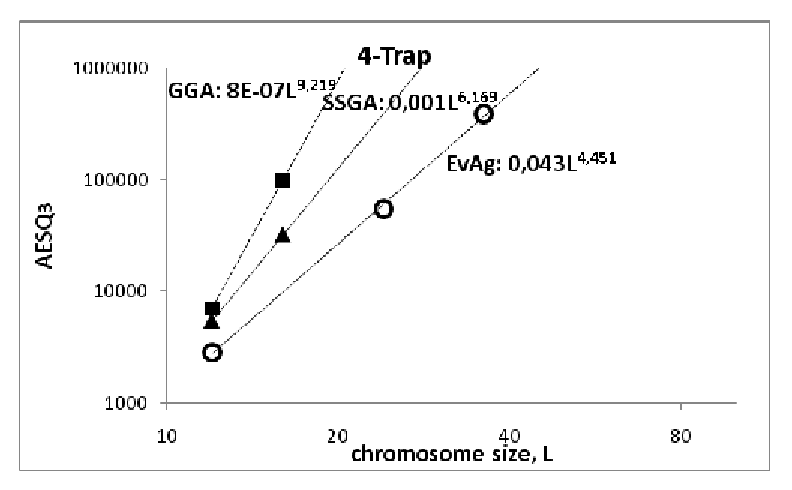
\includegraphics[width=2.9in]{4trapq3es}}
\caption{Scalability in trap functions based on the population tuning algorithm and the selectorecombinative versions of the generational GA (GGA), steady-state GA (SSGA) and the Evolvable Agent (\evag). On the left the estimated population sizes $N$ and the evaluations to solution in third quartile $AESQ_3$ on the right. Results are obtained by bisection and depicted in a {\it log-log} scale as a function of the length of the chromosome, $L$.}
\label{fig:popq3es}
\end{figure*}
%%%%%%%%%%%%%%%%%%%%%%%%%%%%%%%

The first conclusion that can be easily drawn from results is a better scalability of the \evag approach with respect to the population size, specially when the problem difficulty increases from 2 to 4-trap. That is, increasing the problem difficulty makes the GGA and SSGA face extreme difficulties to track the problem optimum, thus requiring a higher population size $N$ to prevent that the algorithm gets stuck in
local optima. From a computational perspective, this fact can be translated  into a more efficient use of the running platform since the \evag approach will require a smaller amount of computational resources. Additionally, results on $AESQ_3$ are clearly correlated to the population size, SSGA scales better than GGA and it is roughly similar to \evag in 2 and 3-trap. Nevertheless, as the problem difficulty increases to 4-trap, \evag scales clearly better.

%%%%%%%%%%%%%%%%%%%%%%%%%%%%%%%
\begin{figure*}[!htpb]
\centering
\centering
\subfigure{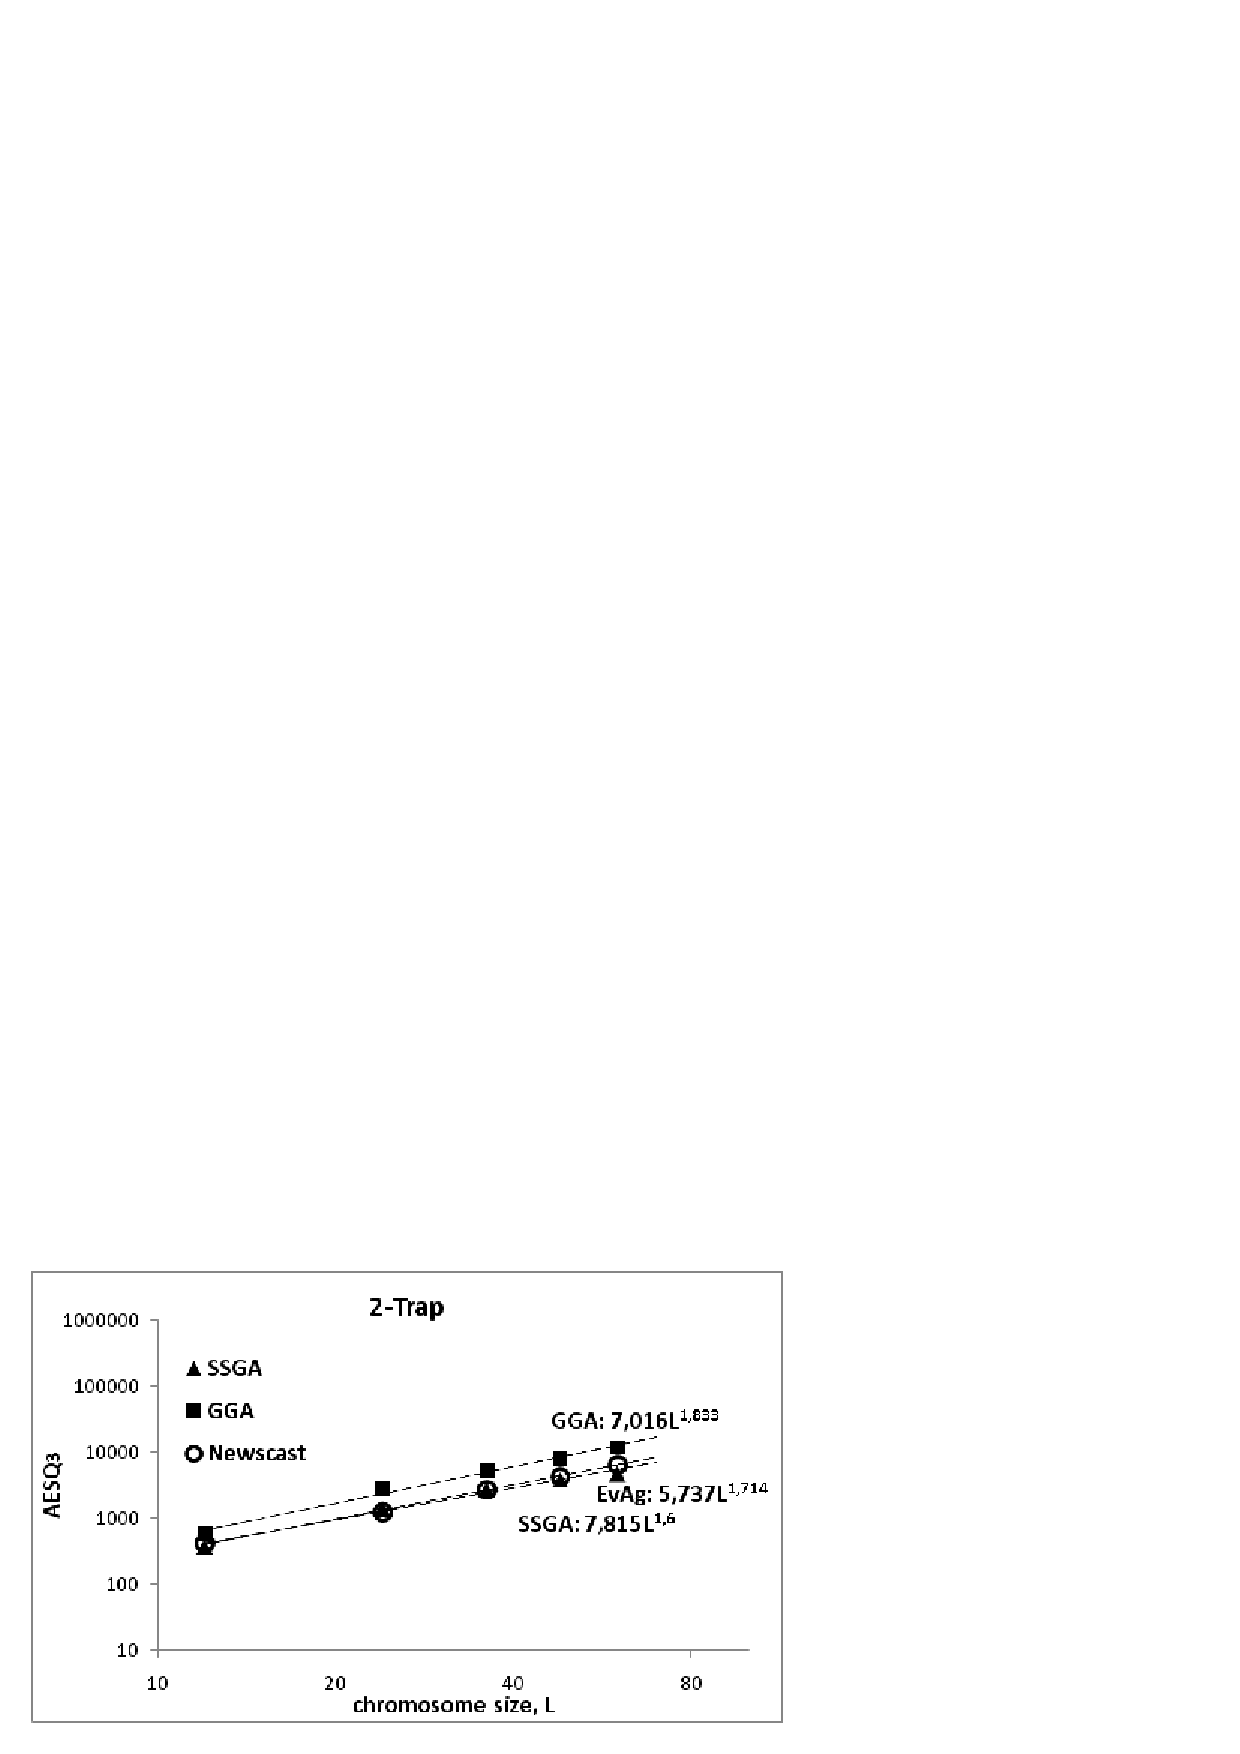
\includegraphics[width=0.6\textwidth]{2trapq3esmut}} \\
\subfigure{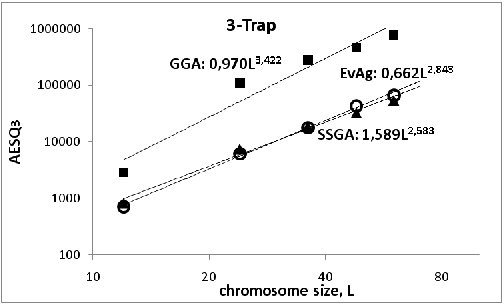
\includegraphics[width=0.6\textwidth]{3trapq3esmut}}\\
\subfigure{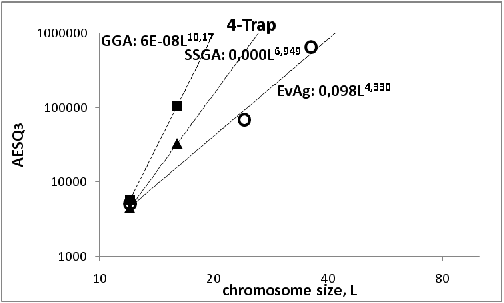
\includegraphics[width=0.6\textwidth]{4trapq3esmut}}
\caption{Reproduction of the results in Figure \ref{fig:popq3es} with
  mutation switched on.}
\label{fig:popq3esmut}
\end{figure*}
%%%%%%%%%%%%%%%%%%%%%%%%%%%%%%%

In order to gain some insight on the influence of mutation in the scalability order, we consider a more realistic GA set-up by switching mutation on. This implies that we have to specify values for the mutation rate parameter $p_m$. Strictly speaking, we should also recalibrate population sizes, since the bisection method only gives 
good estimates for selectorecombinative GAs. However, an extensive parameter sweep goes far beyond the scope of this thesis and therefore we will use the common ``$\frac{1}{L}$ heuristic'' for setting the mutation rates and keep the population sizes that were used in the first series of experiments. Obviously, in this case we only need to look at the $AESQ_3$ results. The outcomes of these experiments are shown in Figure \ref{fig:popq3esmut} in which curves appear shifted with respect to the selectorecombinative version in Figure \ref{fig:popq3es} but approximately keeping the same scalability order. Table \ref{table:orders} compares such estimated complexity orders with mutation switched off and on, showing that mutation does not alter the order in algorithm performance, and exponents are roughly the same, with only the constant in the power law changing.


%%%%%%%%%%%%%%%%%%%%%%%%%%%%%%%%%%%%%%%%%%%%%%%%%%%%%%%%%%%%%%
\begin{table*}[htbp]
\centering
{\small
\begin{tabular}{c|c|c||c |c||c| c|}
&\multicolumn{2}{|c|}{GGA}&\multicolumn{2}{|c|}{SSGA}&\multicolumn{2}{|c|}{\evag}\\
&\multicolumn{2}{|c|}{Mutation}&\multicolumn{2}{|c|}{Mutation}&\multicolumn{2}{|c|}{Mutation}\\
&off&on&off&on&off&on\\
\hline
2-Trap& O($L^{1.804}$)) & O($L^{1.833}$) & O($L^{1.607}$) & O($L^{1.6}$) & O($L^{1.738}$) & O($L^{1.714}$) \\
3-Trap& O($L^{3.24}$) & O($L^{3.422}$) & O($L^{2.454}$) & O($L^{2.583}$) & O($L^{2.498}$) & O($L^{2.843}$) \\
4-Trap& O($L^{9.219}$) & O($L^{10.17}$) & O($L^{6.169}$) & O($L^{6.949}$) & O($L^{4.451}$) & O($L^{4.33}$) \\
\hline
\end{tabular}
}
\caption{ Complexity orders of the $AESQ_3$ scalability in O notation.\label{table:orders}}
\end{table*}
%%%%%%%%%%%%%%%%%%%%%%%%%%%%%%%%%%%%%%%%%%%%%%%%%%%%%%%%%%%%%%

%%% To hold our claims on the best scalability of the \evag approach and having no optimal methods for estimating the population size in GAs with mutation, we focus in the last series of experiments on equally parameterized algorithms with mutation switched on (settings in table \ref{table:thirdserie}). 
%%% replaced entirely by the following

\subsection{Analysis of the algorithmic convergence}
\label{cap5:testcase1:conver}
%%%%%%%%%%%%%%%%%%%%%%%%%%%%%%%%%%%%%%%%%%%%%%%%%%%%%%%%


In the second series of experiments we try to gain more detailed insights in the differences between the three approaches to population management using mutation. To this end, we run the GGA, SSGA, and \evag models using the same settings on a problem instance as summarised in Table \ref{table:sca_secondserie} (recall that in the previous experiments, GGA, SSGA, and \evag used different population sizes on any given problem instance). We choose large instances of each problem under study for this purpose (i.e. $L=36$ in 4-trap, $L=99$ in 3-trap and $L=400$ in 2-trap), where the differences in scalability between the approaches are most visible. 

To estimate the population sizes and the maximum number of evaluations in each case, we have used the scalability orders for the selectorecombinative \evag on the previous series, e.g. $L=99$ in 3-trap will require a population size of $1.098L^{1.479}=942$ and a maximum number of evaluations of  $1.974L^{2.498}=190740$. With these settings, switching mutation on implies that such values are oversized for the \evag approach since mutation represents a new source of diversity, however, the highest scalability orders of SSGA and GGA indicate that such population sizes will remain undersized for both approaches.



%%%%%%%%%%%%%%%%%%%%%%%%%%%%%%%%%%%%%%%%%%%%%%%%%%%%%%%%
\begin{table}[htbp]
\centering
{\scriptsize
\begin{tabular}{r l}
\multicolumn{2}{l}{\textbf{Trap instances}}\\
\hline
2-Trap & \\
Individual Length ($L$) & $400$\\
Population size & 660\\
Termination Condition & Max. Eval. =144700 \\
3-Trap & \\
Individual Length ($L$) & $99$\\
Population size & 942\\
Termination Condition & Max. Eval. =190740 \\
4-Trap & \\
Individual Length ($L$) & $36$\\
Population size & 600\\
Termination Condition & Max. Eval. =393000 \\
&\\
\multicolumn{2}{l}{\textbf{GA settings}}\\
\hline
GA & SSGA \\
&GGA\\
& \evag \\
Selection of Parents & Binary Tournament\\
Recombination & Uniform crossover, $p_c = 1.0$ \\
Mutation & Bit-flip mutation, $p_m = \frac{1}{L}$\\
&\\
\multicolumn{2}{l}{\textbf{Newscast settings}}\\
\hline
Cache size & 20\\

\end{tabular}
}
\caption{Test-case 1: Parameters of the experiments for the analysis of convergence.\label{table:sca_secondserie}}
\end{table}
%%%%%%%%%%%%%%%%%%%%%%%%%%%%%%%%%%%%%%%%%%%%%%%%%%%%%%%%





%%%%%%%%%%%%%%%%%%%%%%%%%%%%%%%
\begin{figure}[!htpb]
\centering
\subfigure{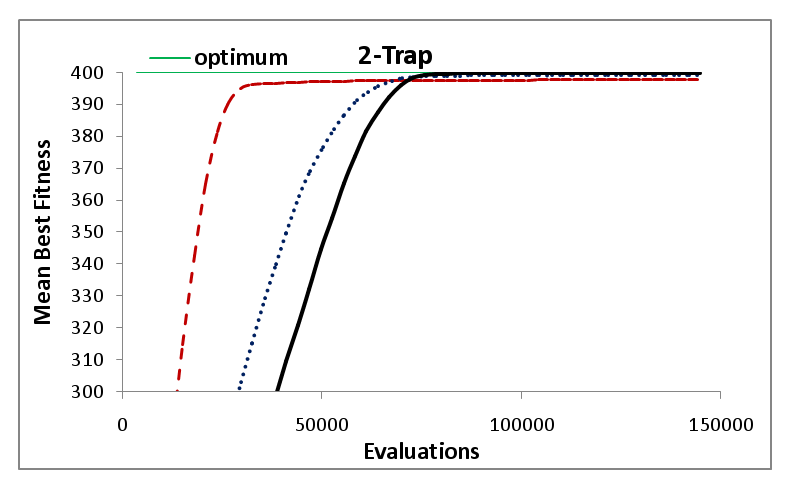
\includegraphics[width=2.9in]{2traplargebestfitness}}
\hspace{1pt}
\subfigure{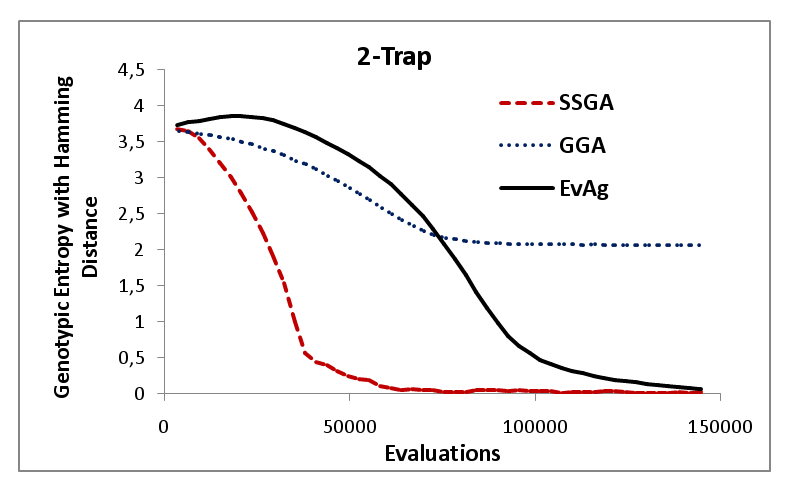
\includegraphics[width=2.9in]{2traplargeentropy}} \\
\subfigure{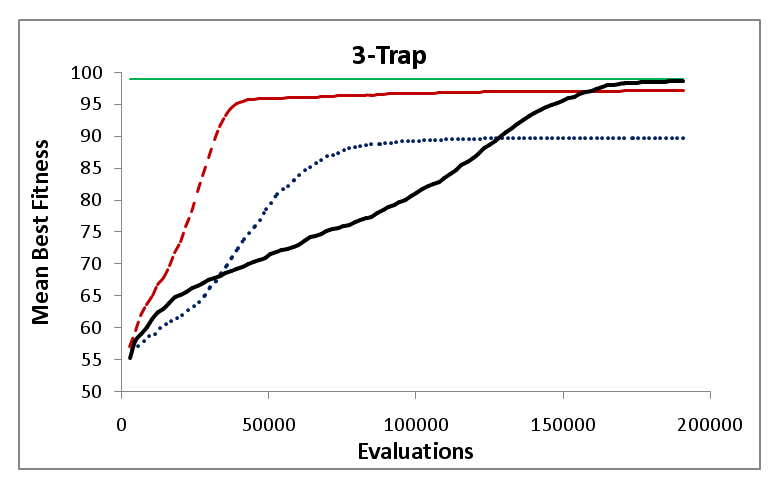
\includegraphics[width=2.9in]{3traplargebestfitness}}
\hspace{1pt}
\subfigure{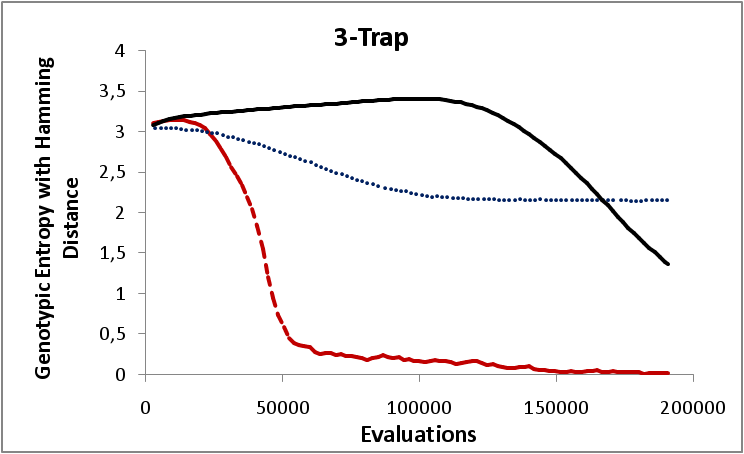
\includegraphics[width=2.9in]{3traplargeentropy}}\\
\subfigure{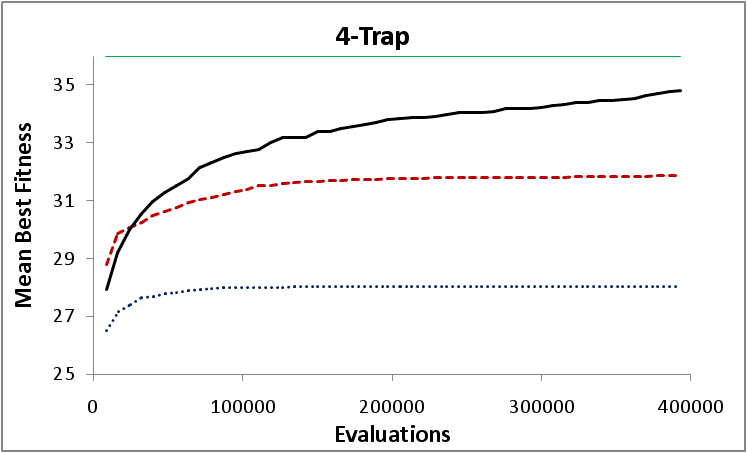
\includegraphics[width=2.9in]{4trapbestfitness}}
\hspace{1pt}
\subfigure{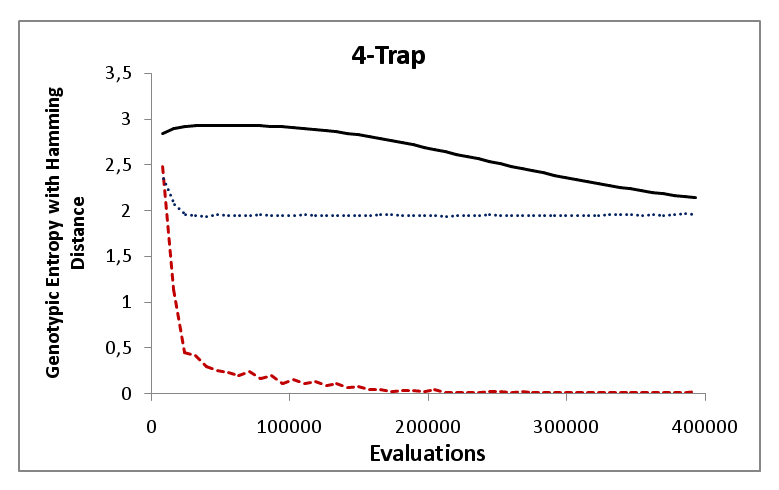
\includegraphics[width=2.9in]{4trapentropy}}
\caption{Test-case 1: Best fitness convergence ({\em left}) and evolution of the
  diversity expressed as the entropy based on the Hamming distances
  between the genotypes ({\em right}). Graphs plotted represent the
  average of 50 independent runs.} 
\label{fig:testcase1convergence}
\end{figure}
%%%%%%%%%%%%%%%%%%%%%%%%%%%%%%%

The results in Figure \ref{fig:testcase1convergence} show that the fitness of the SSGA and GGA approaches stagnates
at early stages of the search in the different instances. Despite the SSGA performing a more
exploitative search than the GGA, as shown by the genotypic entropy
converging to zero, both cases lost track of the optimum, a fact that
might be explained by
an undersized population size. On the other hand, the evolution of
diversity of the \evag approach indicates that the algorithm converges to the optimum in 2 and 3-trap and is still converging in 4-trap when the termination criterion is met. In this last case, it is straightforward to see that the population size is oversized since a selectorecombinative \evag is able to find the optimum in such number of evaluations. Given that the three approaches are equally
parametrised, it is within the spatially structured scheme of reproduction of the \evag model where the
genetic diversity is preserved at a higher level and consequently the
population size $N$ can be reduced. Hence, the \evag approach scales
better on difficult problems. With a lower optimal $N$, \evag needs
fewer evaluations to reach the optimum when compared to panmictic
GAs.




\subsection{Statistical analysis}
\label{cap5:testcase1:statisticalanalysis}
%%%%%%%%%%%%%%%%%%%%%%%%%%%%%%%%%%%%%%%%%%%%%%%%%%%%%%%%

The results shown in the previous Section are analysed in Table \ref{table:testcase1normality} using the Anderson-Darling test to refute the null hypothesis on the normality of the data. The small p-values at the best fitness distributions show that results do not follow a normal distribution. This way, a non-parametric Wilcoxon test is used to compare the quality of fitness between the \evag and the SSGA and GGA approaches.


%%%%%%%%%%%%%%%%%%%%%%%%%%%%%%%%%%%%%%%%%%%%%%%%%%%%%%%%%%%%%%
\begin{table*}[htbp]
\centering
{\tiny
\begin{tabular}{|c|c|c|c|}
\hline
{\it Problem Instance}&{\it Algorithm}&{\it Anderson-Darling }&{\it Normal distribution?}\\
\hline
{\bf Trap2}	&GGA			&	A=3.5 p-value=6.1e-09	&no\\
		&SSGA			&	A=1.8 p-value=6.6e-05	&no\\
&\evag &        A=17 p-value<2.2e-16    &no\\
\hline
{\bf Trap3}	&GGA			& A=0.9   p-value=0.01      &no\\
&SSGA			& A=1.8   p-value=9.9e-05   &no\\

&\evag      & A=11.7  p-value<2.2e-16   &no\\
\hline
{\bf Trap4}	&GGA			&   A=2.4 p-value=2.035e-06 &no\\
&SSGA			&	A=1.2 p-value=0.002     &no\\
&\evag      &   A=12 p-value<2.2e-16    &no\\
\hline
\end{tabular}
}
\caption{Anderson-Darling test on the normality of the best fitness distributions. Results are obtained over 50 independent runs. We have considered $p-values > 0.1$ for a distribution to be normal.\label{table:testcase1normality}}
\end{table*}
%%%%%%%%%%%%%%%%%%%%%%%%%%%%%%%%%%%%%%%%%%%%%%%%%%%%%%%%%%%%%%


 Table \ref{table:testcase1comparative} presents the Wilcoxon analysis of the data showing significant differences between the \evag and canonical approaches in all the problem instances. Therefore, it can be concluded that \evag outperforms SSGA and GGA when tackling large instances of trap functions.


%%%%%%%%%%%%%%%%%%%%%%%%%%%%%%%%%%%%%%%%%%%%%%%%%%%%%%%%%%%%%%
\begin{table*}[htbp]
\centering
{\tiny
\begin{tabular}{|c|c|c|c|c|}
\hline
{\it Problem Instance}&{\it Algorithm}&{\it Avg. Fitness $\pm\sigma$ }&{\it Wilcoxon Test }&{\it Significantly different?}\\
\hline
{\bf Trap2}	&GGA				&	399.08$\pm$1.01		&	W=624 p-value=1.637e-07	&yes\\
L=400		&SSGA			&	397.8$\pm$1.56		&	W=142 p-value<2.2e-16	&yes\\
N=660		&&&&\\
M. Eval.= 144700&{\bf \evag}&{\bf 399.92$\pm$0.27}&-&-\\
\hline
{\bf Trap3}	&GGA				&	89.78$\pm$2.8	&W=0 p-value<2.2e-16&yes\\
L=99		&SSGA			&	97.16$\pm$1.46	&W=402 p-value=3.623e-10&yes\\
N=942		&&	&&\\
M. Eval.= 190740&{\bf \evag}&{\bf 98.72$\pm$0.60}&-&-\\
\hline

{\bf Trap4}	&GGA				&	28.02$\pm$0.14	&W=2500 p-value < 2.22e-16	&yes\\
L=36		&SSGA			&	31.88$\pm$1.15	&W=2476 p-value<2.22e-16&yes\\
N=600		&&&&\\
M. Eval.= 393000&{\bf \evag}&{\bf 34.82$\pm$0.66}&-&-\\
\hline
\end{tabular}
}
\caption{Wilcoxon test comparing the best fitness distributions of equally parametrised SSGA, GGA and \evag in 2,3 and 4-trap. Results are obtained over 50 independent runs.\label{table:testcase1comparative}}
\end{table*}
%%%%%%%%%%%%%%%%%%%%%%%%%%%%%%%%%%%%%%%%%%%%%%%%%%%%%%%%%%%%%%








%%%%%%%%%%%%%%%%% 
\subsection{Summary}
%%%%%%%%%%%%%%%%% 

The \evag model has been proved to have good scalability on trap functions with search landscapes of different degrees of difficulty. We found that \evag scales better than a GGA and an SSGA that only differ from it in the population structure. Based on various scenarios with and without mutation we can conclude that \evag needs fewer evaluations to reach a solution in addition to requiring smaller populations. The improvement is much more noticeable as the problem difficulty increases showing thereby the adequacy of the P2P approach for tackling large instances of difficult problems.  These results are specially remarkable in the deceptive case for a BB size of $4$. It illustrates the good scalability of the parallel approach when tackling difficult problems.

To gain more detailed insights, the runtime behaviour of equally parametrised \evagc SSGA, and GGA approaches have been analysed on large problem instances where the differences of scalability are more outstanding. The results show that \evag can maintain higher population diversity and better progress in fitness. As a consequence, an oversized population for the \evag model still remains undersized for the canonical approaches that get lost in local optima.



\clearpage
%%%%%%%%%%%%%%%%%%%%%%%%%%%%%%%%%%%%%%%%%%%%%%%%%%%%%%%%%%%%%
\section{Test-Case 2: Influence of the population structure on the algorithm performance}
\label{sec:testcase2}
%%%%%%%%%%%%%%%%%%%%%%%%%%%%%%%%%%%%%%%%%%%%%%%%%%%%%%%%%%%%%

As described in Section \ref{sec:evag}, the \evag model imposes no restrictions on the choice of a population structure. Within that context, the newscast protocol has been considered throughout this thesis in order to allow a decentralised execution of the approach in a P2P system. Nevertheless, different structures will influence the dynamics of the algorithm in a different way and therefore, its algorithmic performance. Hence, the aim of this test-case is the comparison of performances of the approach using three different population structures. To that aim, the ring and the Watts-Strogatz method explained in Section \ref{sec:structurecomplex} have been considered for comparison against newscast (Figure \ref{fig:testcase2} shows snapshots for the different population structures). 



\begin{figure*}[htbp]
\centerline{\subfigure{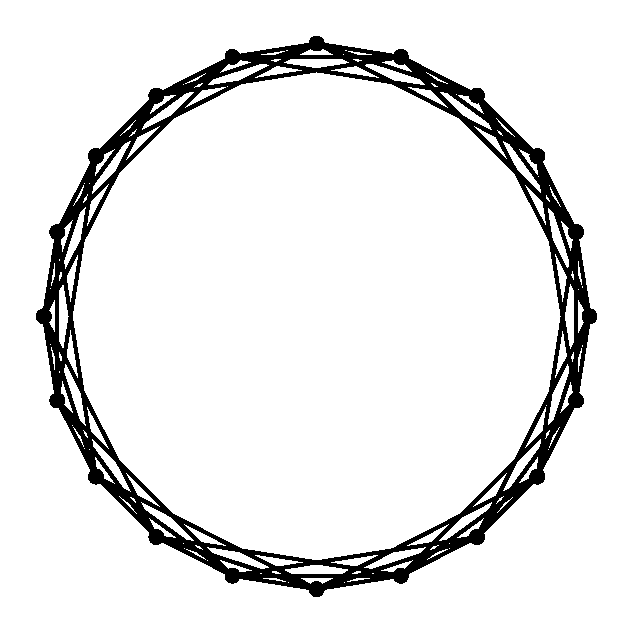
\includegraphics[width=1.5in]{WS-20-0000}
}
\hfil
\subfigure{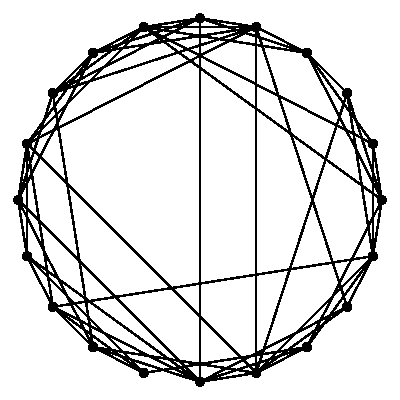
\includegraphics[width=1.5in]{WS-20-0200}
}
\hfil
\subfigure{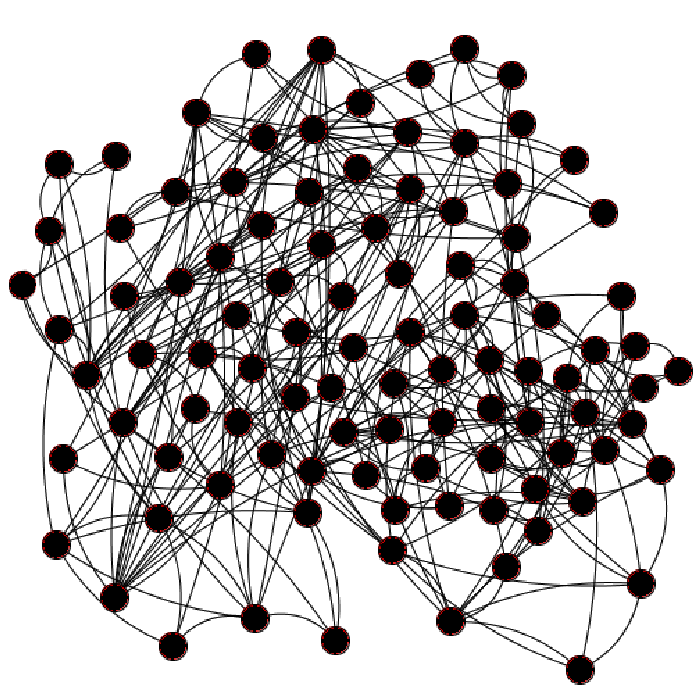
\includegraphics[width=1.5in]{newscastgraph}
}}
\caption{ From left to right: ring, Watts-Strogatz and newscast population structures.
}
\label{fig:testcase2}
\end{figure*}

We have chosen a ring population structure as an instance to compare the performance of regular lattices against newscast since most of the works in the literature considering fine-grained approaches use to focus in regular lattices (some examples have been already mentioned in this thesis including \cite{asparagos1989,alba:cga,tomassini,dagt04,giacobini:gecco04,giacobini:regular}).  The main reason for such a choice is that the bisection method is not applicable for some other regular lattices such as a toroid or a grid in which the rectangular dimensions of the topology do not allow doubling the size of the population in the process of estimating the correct size.

In addition, the Watts-Strogatz method represents an easy and understandable model for creating a  small-world population structure. This way, it will be possible to compare two different methods (i.e. Watts-Strogatz and newscast) for generating the same sub-type of complex network. The interest here goes a step further than in the case of the ring since there are many P2P protocols designed to work as small-world networks. Therefore, we aim to establish whether the properties on scalability of the newscast population structure lie in its small-world structure so that may extend to other protocols implementing the same kind of topologies (e.g. Gnutella 0.4 \cite{gnutella04} or any DHT \cite{chord,pastry,tapestry,can}).


Figure \ref{fig:takeovernwsr} depicts the influence of the three methods in the environmental selection pressure by their respective takeover times. It shows both small-world populations inducing similar pressures in spite of being a bit stronger in the case of newscast. Meanwhile, the ring structure shows a delay in the takeover time given that the network diameter is larger at such a kind of topology.

\begin{figure*}[htbp]
\centerline{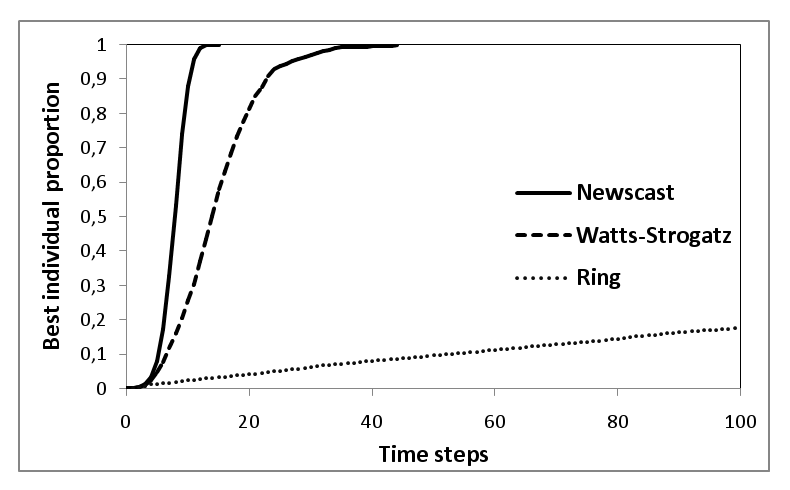
\includegraphics[width=0.7\textwidth]{takeovernwsr}}
\caption{Takeover time curves in a ring, Watts-Strogatz with $p=0.2$ and newscast population structures. All results averaged from 50 independent runs, for a population size of $n=1600$ and binary tournament. }
\label{fig:takeovernwsr}
\end{figure*}



\subsection{Scalability analysis}
%%%%%%%%%%%%%%%%%%%%%%%%%%%%%%%%%%%%%%%%%%%%%%%%%%%%%%%%

The following experiment aims to compare the influence of previous decentralised population structures on the scalability of the \evag model when tackling trap functions. Table \ref{table:testcase2_sca_parameters} summarises the settings in these series including the ring, Watts-Strogatz and newscast.



%%%%%%%%%%%%%%%%%%%%%%%%%%%%%%%%%%%%%%%%%%%%%%%%%%%%%%%%
\begin{table}[htbp]
\centering
{\scriptsize
\begin{tabular}{r l}
\multicolumn{2}{l}{\textbf{Trap instances}}\\
\hline
BB size & $2, 3, 4$\\
Individual Length ($L$) & $12, 24, 36, 48, 60$\\
&\\
\multicolumn{2}{l}{\textbf{GA settings}}\\
\hline
GA & selectorecombinative \evag \\
Population size & Tuning algorithm\\
Selection of Parents & Binary Tournament\\
Recombination & Uniform crossover, $p_c = 1.0$ \\
&\\
\multicolumn{2}{l}{\textbf{Population settings}}\\
\hline
Population structure & Ring\\
& Watts-Strogatz, $p=0.2$\\
& Newscast\\
Node degree & 20\\

\end{tabular}
}
\caption{Test-case 2: parameters of the experiments in the analysis of scalability. \label{table:testcase2_sca_parameters}}
\end{table}
%%%%%%%%%%%%%%%%%%%%%%%%%%%%%%%%%%%%%%%%%%%%%%%%%%%%%%%%

Figure \ref{fig:popaestop} depicts the scalability of the population size and the computational effort for the different population structures in 2, 3 and 4-trap functions. Results show that the ring structure is able to scale better than its counterparts with respect to the population size. In that context, the ring has been shown to relax the environmental selection pressure and will consequently preserve the genetic diversity. This way, the population size can be reduced at every instance and the scalability order improves. Nevertheless, the analysis drastically changes with respect to the computational efforts. In such case, the ring population scales worse than the small-world ones requiring therefore a larger time to converge to optimal solutions.

In addition, the comparison between the two small-world methods shows that the scalability of the population size  using the Watts-Strogatz method is slightly better than in the case of newscast. Nevertheless, results are quite similar with respect to the scalability of the computational efforts in which there is no clear trend of an approach outperforming the other when changing the problem landscape difficulty. Taking into account that results are estimations based on the bisection method, such orders of scalability point out that either Watts-Strogatz or newscast perform roughly the same, the newscast approach needing a slightly larger population size than Watts-Strogatz but requiring equivalent times to solution.


%%%%%%%%%%%%%%%%%%%%%%%%%%%%%%%
\begin{figure}[!htpb]
\centering
\centering
\subfigure{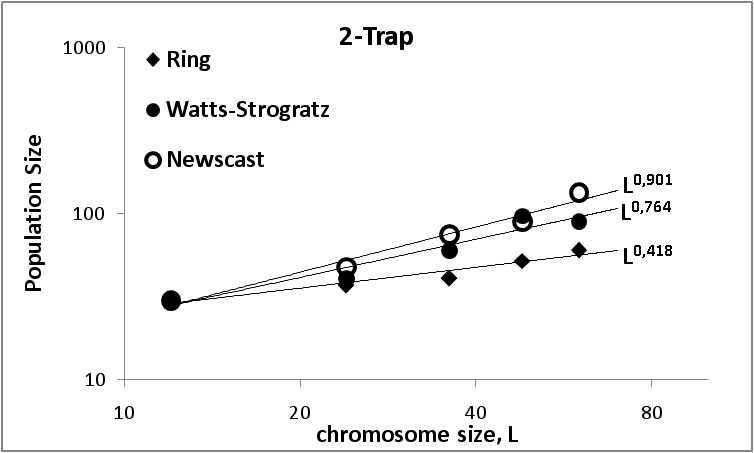
\includegraphics[width=2.9in]{top2trappop}}
\hspace{1pt}
\subfigure{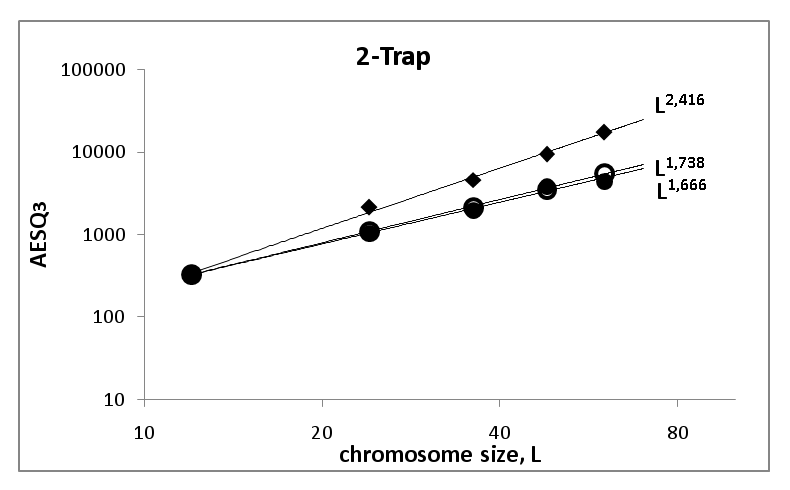
\includegraphics[width=2.9in]{top2trapq3es}} \\
\subfigure{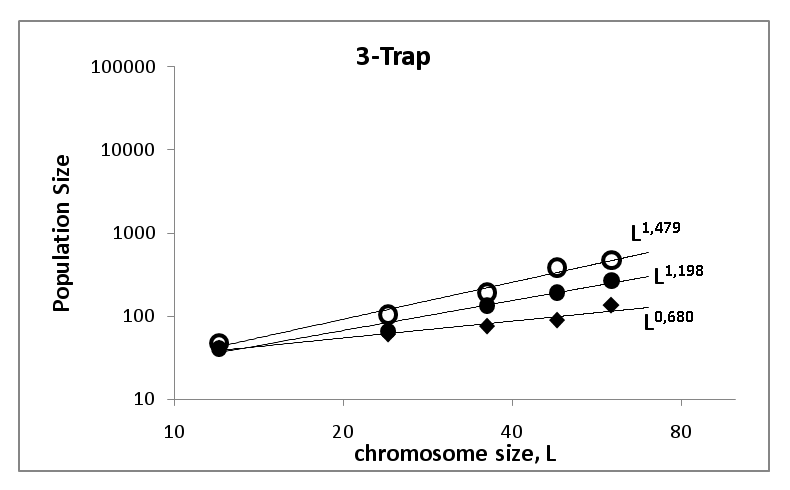
\includegraphics[width=2.9in]{top3trappop}}
\hspace{1pt}
\subfigure{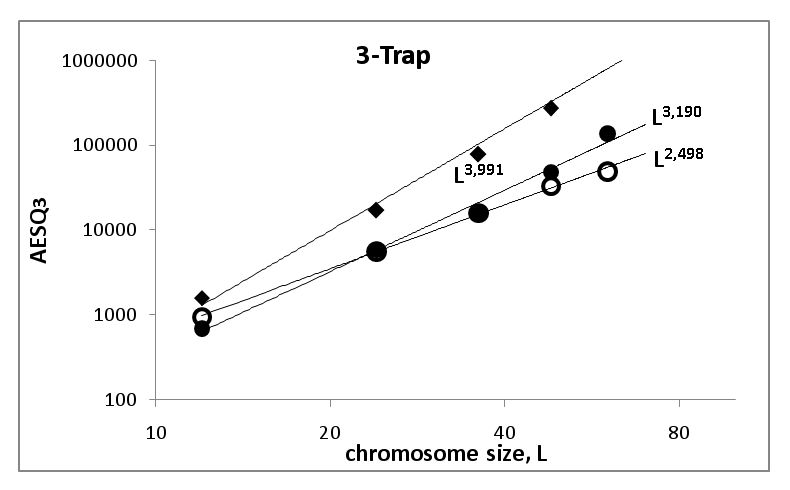
\includegraphics[width=2.9in]{top3trapq3es}}\\
\subfigure{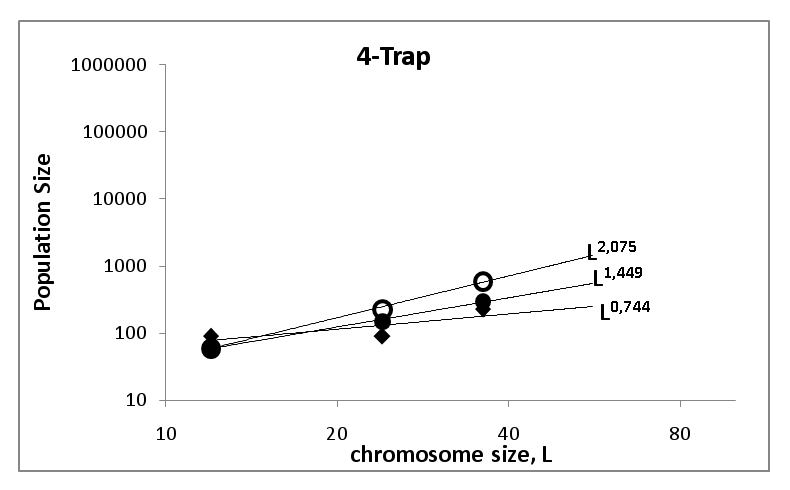
\includegraphics[width=2.9in]{top4trappop}}
\hspace{1pt}
\subfigure{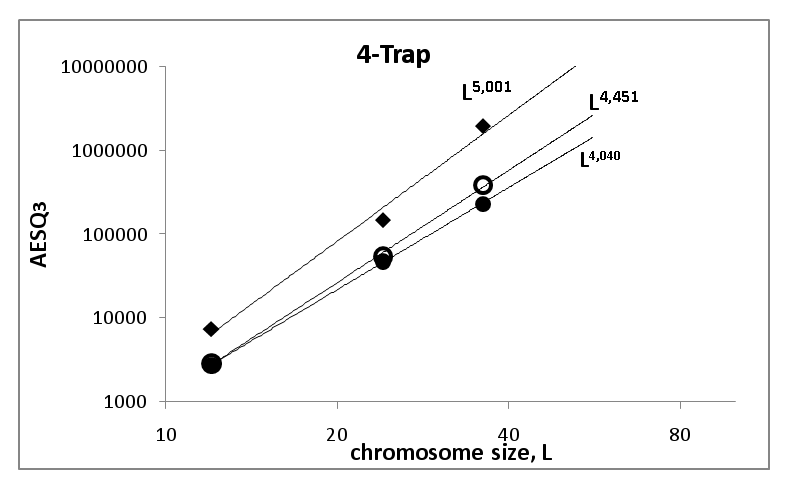
\includegraphics[width=2.9in]{top4trapq3es}}
\caption{Scalability  of the \evag model using a Ring, Watts-Strogatz and Newscast population structures in trap functions for the estimated population sizes $N$ {\em (left)} and the evaluations to solution in third quartile {\em (right)}. Results are obtained by bisection and depicted in a {\em log-log} scale as a function of the length of the chromosome, $L$.}
\label{fig:popaestop}
\end{figure}
%%%%%%%%%%%%%%%%%%%%%%%%%%%%%%%


\clearpage

\subsection{Analysis of the algorithmic convergence}
%%%%%%%%%%%%%%%%%%%%%%%%%%%%%%%%%%%%%%%%%%%%%%%%%%%%%%%%

This section analyses the convergence of the \evag approach in large instances of 2, 3 and 4-trap for different population structures. All settings for the experiments are summarised in Table \ref{table:testcase2sca_secondserie}. In order to establish the population sizes and the maximum number of evaluations for the different instances, we have chosen previous values obtained by bisection for the selectorecombinative \evag using newscast. The aim here is to provide better insights on the algorithmic convergence for the three topologies when the \evag model is equally parametrised.


%%%%%%%%%%%%%%%%%%%%%%%%%%%%%%%%%%%%%%%%%%%%%%%%%%%%%%%%
\begin{table}[htbp]
\centering
{\scriptsize
\begin{tabular}{r l}
\multicolumn{2}{l}{\textbf{Trap instances}}\\
\hline
2-Trap & \\
Individual Length ($L$) & $60$\\
Population size & 135\\
Termination Condition & Max. Eval. = 5535\\
3-Trap & \\
Individual Length ($L$) & $60$\\
Population size & 480\\
Termination Condition & Max. Eval. =49920\\
4-Trap & \\
Individual Length ($L$) & $36$\\
Population size & 600\\
Termination Condition & Max. Eval. =393000 \\
&\\
\multicolumn{2}{l}{\textbf{GA settings}}\\
\hline
GA & \evag \\
Selection of Parents & Binary Tournament\\
Recombination & Uniform crossover, $p_c = 1.0$ \\
Mutation & Bit-flip mutation, $p_m = \frac{1}{L}$\\
&\\
\multicolumn{2}{l}{\textbf{Population settings}}\\
\hline
Population structure & Ring\\
& Watts-Strogatz\\
& Newscast\\
Node degree & 20\\

\end{tabular}
}
\caption{Test-Case 2: Parameters of the experiments for the analysis of convergence.\label{table:testcase2sca_secondserie}}
\end{table}
%%%%%%%%%%%%%%%%%%%%%%%%%%%%%%%%%%%%%%%%%%%%%%%%%%%%%%%%

Figure \ref{fig:testcase2convergencetop} shows both small-world approaches having a better progress in fitness than the ring one in every instance under study. In fact, either Watts-Strogatz or newscast reach the same qualities in solutions at the maximum number of evaluations.

In addition, results for the genotypic entropy provide some keys on the influence of the population structure on the algorithm. The ring preserves the genetic diversity at a higher level than its counterparts delaying this way the convergence of fitness. Besides, the same shape in curves of the Watts-Strogatz and newscast approaches indicate that both population structures belong to a same kind of topology. Nevertheless, newscast promotes a stronger selection pressure as was shown by the takeover time curves in Figure \ref{fig:takeovernwsr}.


%%%%%%%%%%%%%%%%%%%%%%%%%%%%%%%
\begin{figure}[!htpb]
\centering
\subfigure{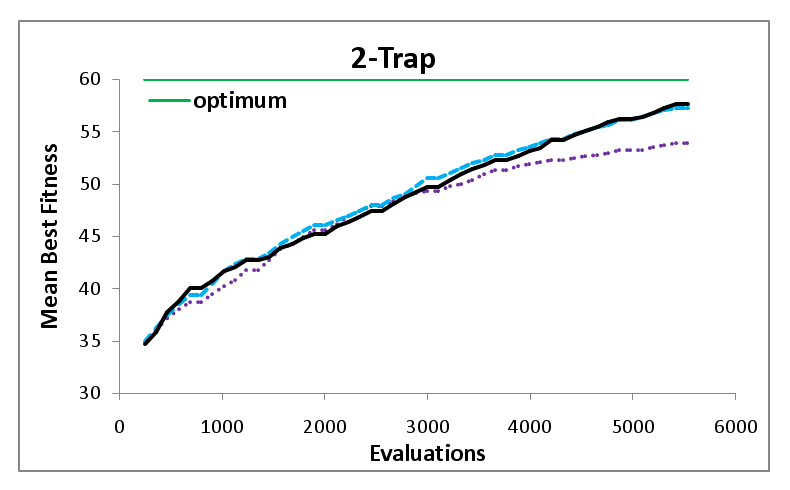
\includegraphics[width=2.9in]{top2trapbestfitness}}
\hspace{1pt}
\subfigure{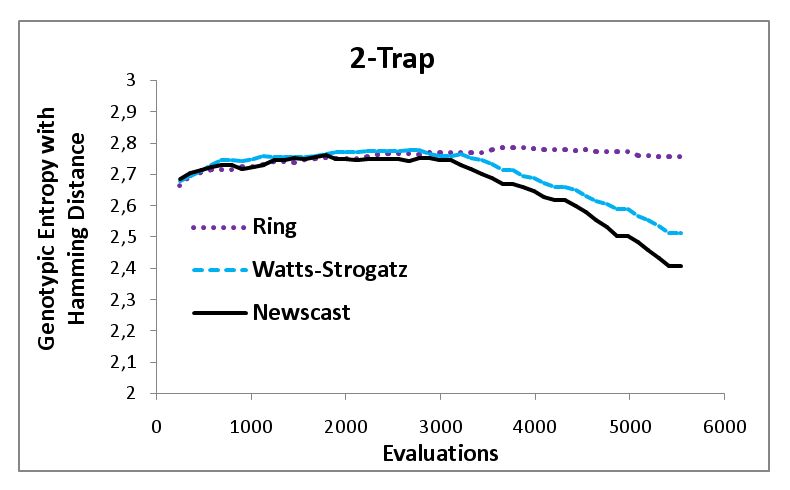
\includegraphics[width=2.9in]{top2trapentropy}} \\
\subfigure{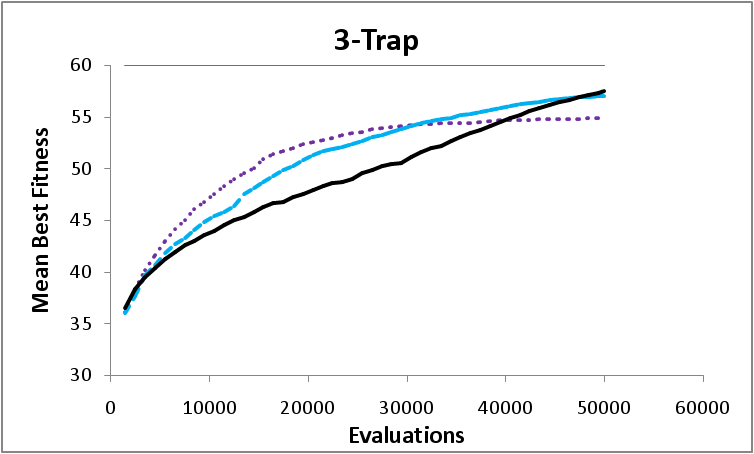
\includegraphics[width=2.9in]{top3trapbestfitness}}
\hspace{1pt}
\subfigure{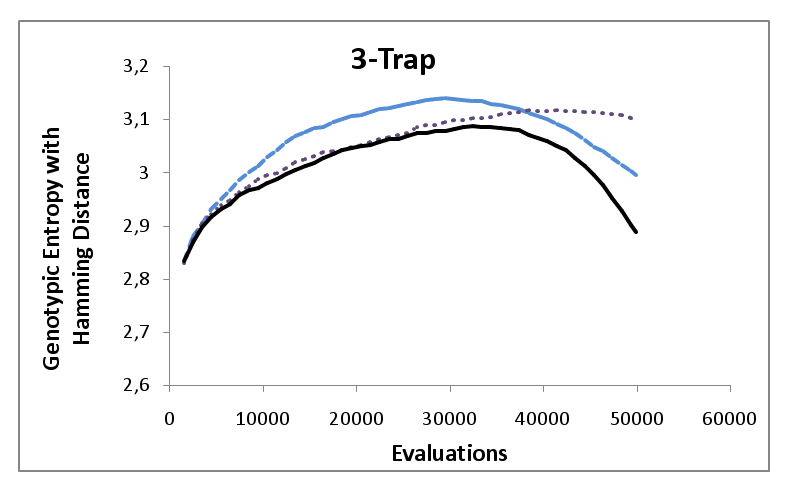
\includegraphics[width=2.9in]{top3trapentropy}}\\
\subfigure{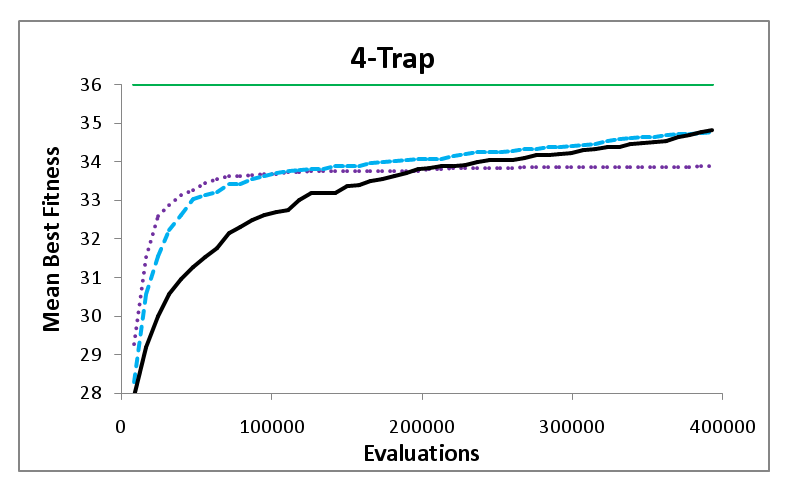
\includegraphics[width=2.9in]{top4trapbestfitness}}
\hspace{1pt}
\subfigure{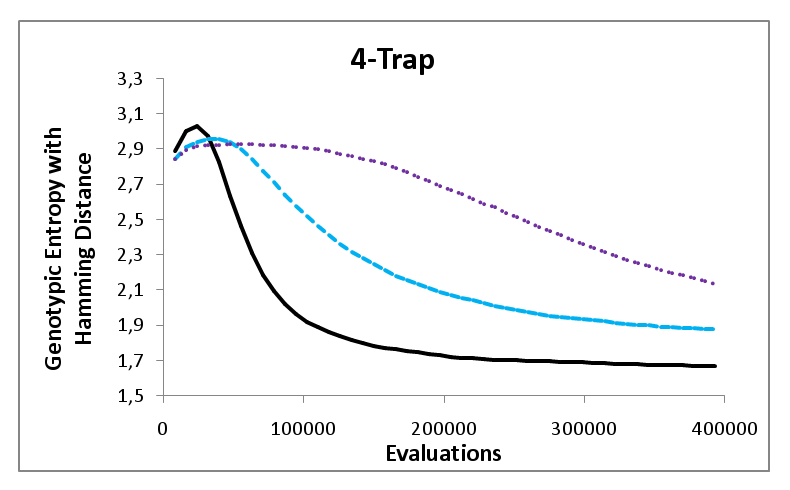
\includegraphics[width=2.9in]{top4trapentropy}}
\caption{Test-Case 2: Best fitness convergence ({\em left}) and evolution of the
  diversity expressed as the entropy based on the Hamming distances
  between the genotypes ({\em right}). Graphs plotted represent the
  average of 50 independent runs.}
\label{fig:testcase2convergencetop}
\end{figure}
%%%%%%%%%%%%%%%%%%%%%%%%%%%%%%%


\subsection{Statistical analysis}
%%%%%%%%%%%%%%%%%%%%%%%%%%%%%%%%%%%%%%%%%%%%%%%%%%%%%%%%

The Wilcoxon analysis in Table \ref{table:comparativerws} shows that differences in fitness between newscast and ring population structures are statistically significant which confirms previous results  on the different convergences of the approaches. Nevertheless, such differences do not appear when comparing newscast with the Watts-Strogatz model in 2 and 4-trap. Additionally, the $p-value=0.045$ in the 3-trap instance points to a close related distribution of fitness between both approaches.

Therefore, the small-world population structures generated by both methods promote equivalent algorithmic performances. This fact is promising for the exploration of other small-world based P2P protocols in the context of the EC paradigm.




%%%%%%%%%%%%%%%%%%%%%%%%%%%%%%%%%%%%%%%%%%%%%%%%%%%%%%%%%%%%%%
\begin{table*}[htbp]
\centering
{\tiny
\begin{tabular}{|c|c|c|c|c|}
\hline
{\it Problem Instance}&{\it Algorithm}&{\it Avg. Fitness $\pm\sigma$ }&{\it Wilcoxon Test }&{\it Significantly different?}\\
\hline
{\bf Trap2}	&				&			&	&\\
L=60		&Ring			&	53.88$\pm$1.21		&	W=2429 p-value=2.22e-16	&yes\\
N=135		&{\bf Watts-Strogatz}&{\bf	57.26$\pm$1.52	}&{\bf W=1386 p-value=0.335	}&{\bf no}\\
M. Eval.= 5535&{\bf Newscast}&{\bf 57.6$\pm$1.38}&-&-\\
\hline
{\bf Trap3}	&				&		& & \\
L=60		&Ring			&	54.9$\pm$0.97	&W=2135 p-value=6.46e-10&yes\\
N=480		&{\bf Watts-Strogatz}&{\bf	57.04$\pm$1.07}&{\bf W=1536 p-value=0.045}&{\bf yes}\\
M. Eval.= 49920&{\bf Newscast}&{\bf 57.5$\pm$2.04}&-&-\\
\hline

{\it Trap4}	&				&		& 	&\\
L=36		&Ring			&	33.88$\pm$0.69	&W=2044 p-value=4.38e-09&yes\\
N=600		&{\bf Watts-Strogatz}&{\bf 	34.78$\pm$0.65	}&{\bf W=1288 p-value=0.77 }&{\bf no}\\
M. Eval.= 393000&{\bf Newscast}&{\bf 34.82$\pm$0.66}&-&-\\

\hline
\end{tabular}
}
\caption{Wilcoxon test comparing the best fitness distribution of the \evag model using a Ring, Watts-Strogatz and Newscast population structures. Results are obtained over 50 independent runs.\label{table:comparativerws}}
\end{table*}
%%%%%%%%%%%%%%%%%%%%%%%%%%%%%%%%%%%%%%%%%%%%%%%%%%%%%%%%%%%%%%


%%%%%%%%%%%%%%%%%%%%%%%%%%%%%%%%%%%%%%%%%%%%%%%%%%%%%%%%%%%%%
\subsection{Summary}
%%%%%%%%%%%%%%%%%%%%%%%%%%%%%%%%%%%%%%%%%%%%%%%%%%%%%%%%%%%%%

In this test-case, we have analysed the \evag model using different decentralised population structures in order to assess their influence on the performance of the algorithm. A ring topology and the Watts-Strogatz method were considered for comparison against the newscast method which allows a decentralised execution of the approach in a P2P system. 

The ring topology has been chosen as the instance to compare regular lattices performances against newscast given that such kind of population structures are commonly used in fine-grained approaches. In addition, the Watts-Strogatz method is an easy method for generating small-world topologies. The aim here is to establish whether population structures based on small-world networks have equivalent performances so that \evag  can be extended to other P2P protocols implementing such a kind of topologies.

Results show that the ring approach needs smaller population sizes than newscast to guarantee a reliable convergence but, in turn, it requires of a larger number of evaluations which translates into larger times to solution. On the other hand, the Watts-Strogatz method exerts a slightly more relaxed selection pressure in the algorithm than newscast, however, results on the computational scalability and on the algorithmic convergence show that both approaches have similar performances that do not present statistical differences in qualities of solutions. Therefore, it can be concluded that both methods promote similar behaviours in the algorithm performance. We find that fact promising since such a property may extend to other small-world based P2P protocols.



\clearpage
%%%%%%%%%%%%%%%%%%%%%%%%%%%%%%%%%%%%%%%%%%%%%%%%%%%%%%%%%%%%%
\section{Test-Case 3: Fault tolerance of the model}
\label{sec:testcase3}
%%%%%%%%%%%%%%%%%%%%%%%%%%%%%%%%%%%%%%%%%%%%%%%%%%%%%%%%%%%%%
As explained in chapter \ref{cap:p2pcompt}, P2P systems are large networks of volatile resources in which the collective dynamics of peers joining and departing from the system is known as \emph{churn}. This way, addressing churn in a P2P EA turns into a requirement of design since failures in peers are inherent to the system.

Following the work by Stutzbach and Rejaie in \cite{Stutzbach06Understanding}, there are two main group-level properties of \emph{churn} characterising the behaviour of every participating peer: The \emph{inter-arrival time} and the \emph{session length}, respectively, the time between two sessions and the time from the beginning to the end of a session. In this test-case, we have assumed that all peers start at the same time with a certain \emph{session length} and avoiding \emph{inter-arrivals}. Therefore, once a peer leaves the system, it does not re-join again so that the system {\em degrades} from the initial configuration.

The \emph{session length}  can be modelled randomly from a Weibull distribution using the following formula:

\begin{equation}\label{eq:weibull}
X = \lambda (-ln(U))^{\frac{1}{k}}
\end{equation}


\noindent
where $U$ is drawn from the uniform distribution, $k$ stands for the shape of the {\em degradation} and $\lambda$ for the time scale. 

In this context, Stutzbach and Rejaie analyse the runtime dynamics of three real P2P systems and conclude that   all {\em session lengths} fit with a Weibull distribution of shape $k \approx 0.40$ but differing on the time dimension $\lambda$. Given that experiments are conducted in a simulator and a simulator cycle represents different time units in real time, $\lambda$ parameter was pre-adjusted to simulate different failure rates in such a way that the system degrades up to $90\%$ in the worst case. In concrete, we use the following values for $\lambda=400,2500$ (depicted in Figure \ref{fig:ccdf}). It shows the Weibull cumulative distribution functions for such values, representing the percentage of remaining nodes at each moment of a experiment (e.g. in the cycle $2000$, $\sim$15\% of the peers remain for $\lambda=400$ and $\sim$75\% for $\lambda=2500$).


%The analysis by Stutzbach and Rejaie on three real P2P systems exposes that the \emph{session length} fit with a shape of $s \approx 0.40$ but the values of $\lambda$ differ. Additionally, the simulator driven experiments define the time unit as a simulator cycle which could apply for different time metrics in real time. Hence, we set-up the following values for $\lambda=1,5,10,\infty$ depicted in Figure \ref{fig:ccdf}. It shows the complementary cumulative distribution functions (CCDF), representing the percentage of remaining nodes at each moment of the experiment for the different values of $\lambda$ (e.g. in the cycle 10, $\sim$8\% of the peers remain for $\lambda=1$ and $\sim$50\% for $\lambda=10$).


%%%%%%%%%%%%%%%%% 
\begin{figure}[!htpb]
\centerline{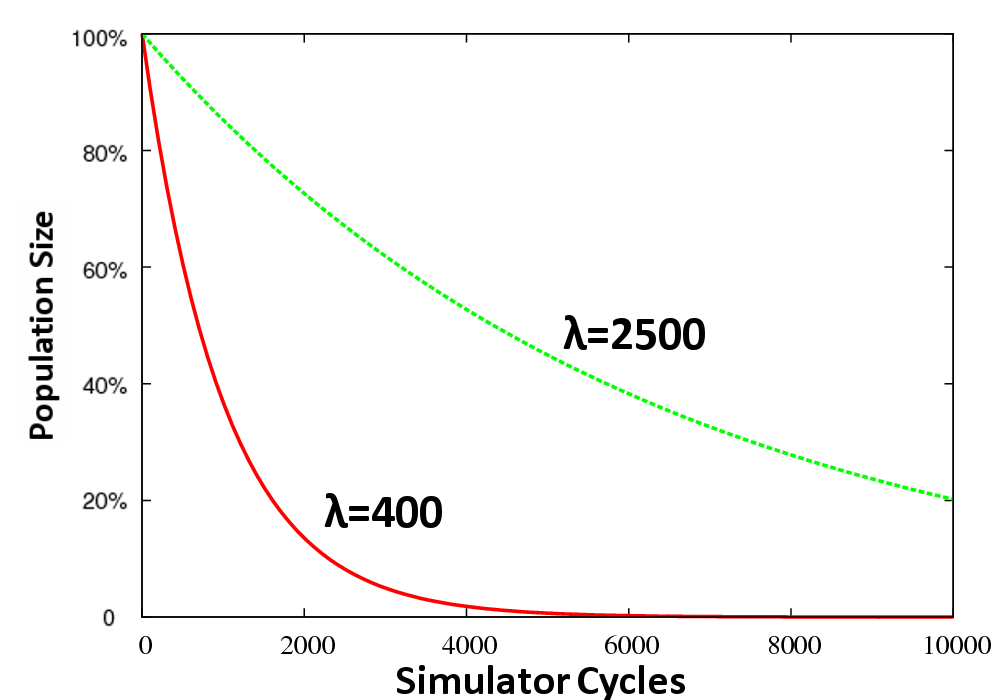
\includegraphics[width=0.7\textwidth]{ccdf}}
\caption{ Complementary cumulative distribution functions for a Weibull distribution in function of the simulator cycles. Percentages are obtained as the ratio between the total number of failures and the initial population size.}
\label{fig:ccdf}
\end{figure}
%%%%%%%%%%%%%%%%% 




\subsection{Scalability analysis}
%%%%%%%%%%%%%%%%%%%%%%%%%%%%%%%%%%%%%%%%%%%%%%%%%%%%%%%%

Using previous {\em degradation} rates, several instances of 2, 3 and 4-trap have been analysed in order to assess the impact of churn in the \evag model. All settings for the experiments are summarised in Table \ref{table:testcase3_sca_parameters}.

This way, there will be three variables affecting the performance of the algorithm: The size of the problem ($L$), which will conduct to a scalability analysis, the intensity of churn ($\lambda$) and the  initial\footnote{Given that the system degrades, the initial population size will not correspond to the final one.} population size ($N$). Being $\lambda$ and $L$ two independent variables under the condition of obtaining a SR of 0.98, the initial population size can be expressed as a function $f(\lambda,L)=N$ and empirically estimated using the bisection method.



%%%%%%%%%%%%%%%%%%%%%%%%%%%%%%%%%%%%%%%%%%%%%%%%%%%%%%%%
\begin{table}[htbp]
\centering
{\scriptsize
\begin{tabular}{r l}
\multicolumn{2}{l}{\textbf{Trap instances}}\\
\hline
BB size & $2, 3, 4$\\
Individual Length ($L$) & $12, 24, 36, 48, 60$\\
&\\
\multicolumn{2}{l}{\textbf{GA settings}}\\
\hline
GA & selectorecombinative \evag \\
Population size & Tuning algorithm\\
Selection of Parents & Binary Tournament\\
Recombination & Uniform crossover, $p_c = 1.0$ \\
&\\
\multicolumn{2}{l}{\textbf{Newscast settings}}\\
\hline
Cache Size & 20\\
&\\
\multicolumn{2}{l}{\textbf{Scenarios of churn}}\\
\hline
$\lambda$ & 400,2500\\
$k$ & 0.4\\

\end{tabular}
}
\caption{Test-case 3: parameters of the experiments in the analysis of scalability. \label{table:testcase3_sca_parameters}}
\end{table}
%%%%%%%%%%%%%%%%%%%%%%%%%%%%%%%%%%%%%%%%%%%%%%%%%%%%%%%%

Figure \ref{fig:popaeschurn} shows the scalability of the population size ($N$) as a function of $L$, that is, $L$ scales and $\lambda$ remains fixed in $f(\lambda,L)=N$. \emph{Churn} does not seem to damage the scalability of the approach since estimated curves $f(\lambda,L)$ roughly follow  the same orders of scalability and  just appear shifted by a constant which is churn dependent. The more intensive the churn, the bigger the constant. In this sense, a small increase on the initial population size is enough to provide resilience to system failures since orders of scalability go from $O(L^{0.901})$ to $O(L^{0.928})$ in 2-trap, $O(L^{1.479})$ to $O(L^{1.799]})$ in 3-trap and are estimated to $O(L^{2.075})$ for any scenario in 4-trap. 


%%%%%%%%%%%%%%%%%%%%%%%%%%%%%%%
\begin{figure}[!htpb]
\centering
\centering
\subfigure{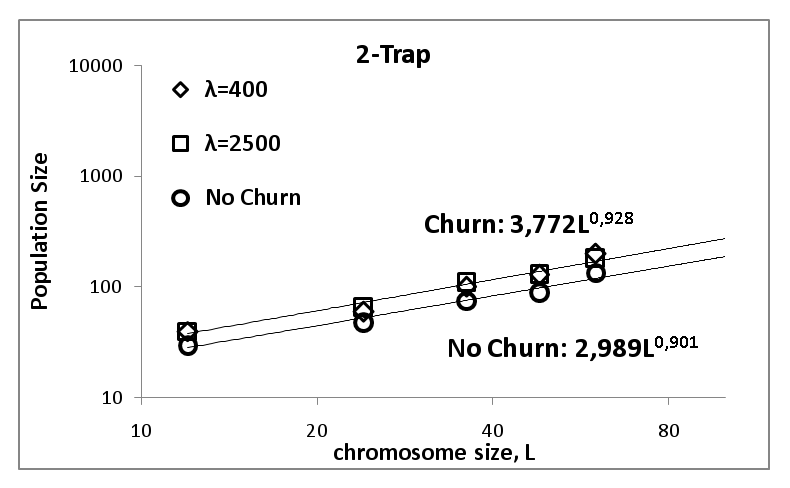
\includegraphics[width=2.9in]{churn2trappop}}
\hspace{1pt}
\subfigure{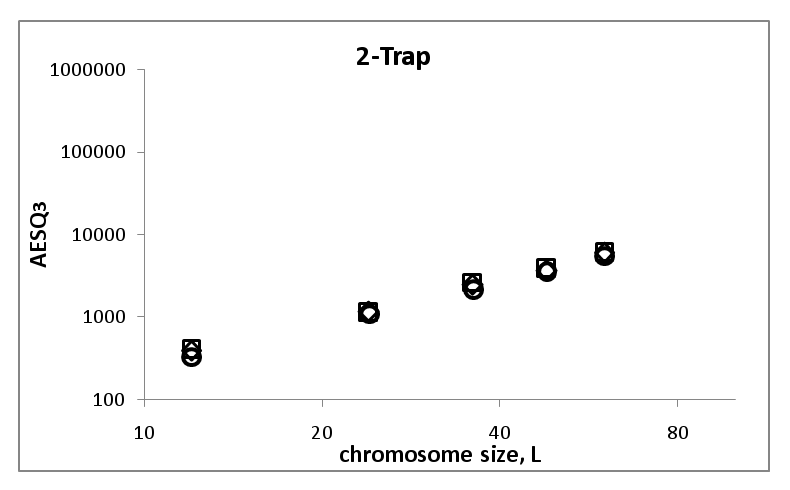
\includegraphics[width=2.9in]{churn2trapq3es}} \\
\subfigure{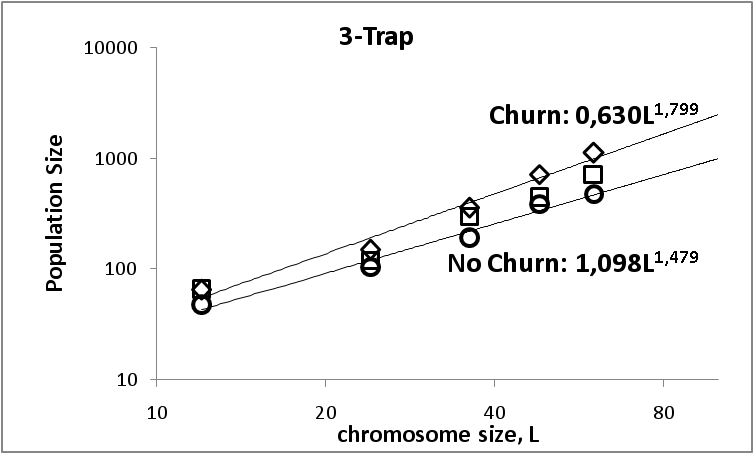
\includegraphics[width=2.9in]{churn3trappop}}
\hspace{1pt}
\subfigure{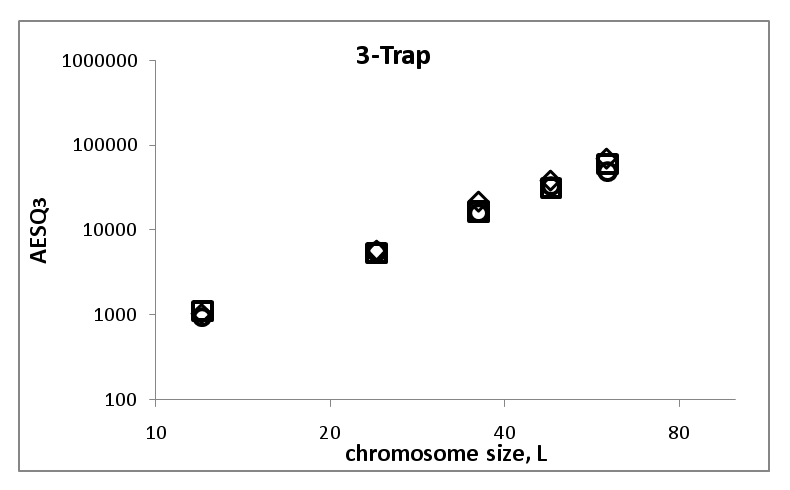
\includegraphics[width=2.9in]{churn3trapq3es}}\\
\subfigure{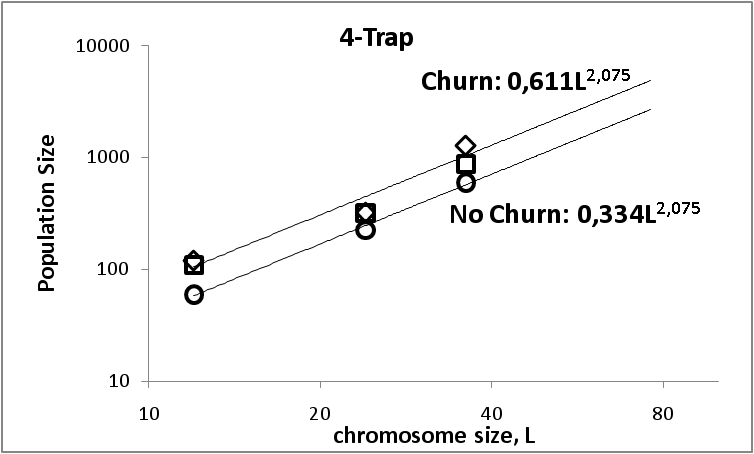
\includegraphics[width=2.9in]{churn4trappop}}
\hspace{1pt}
\subfigure{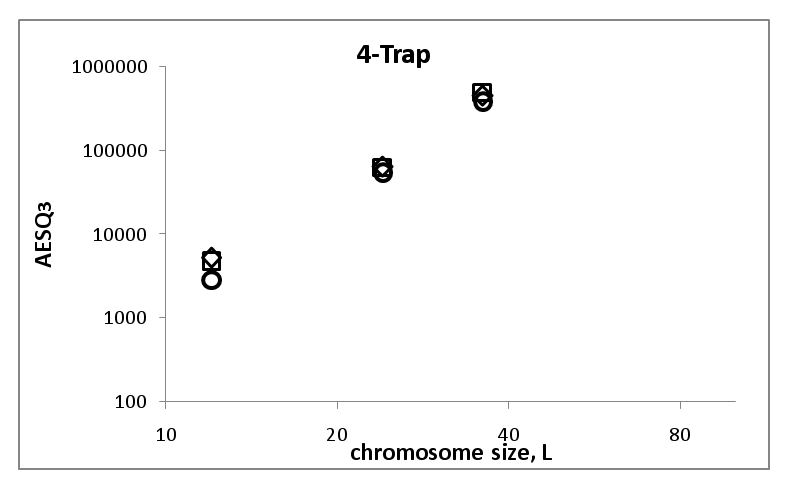
\includegraphics[width=2.9in]{churn4trapq3es}}
\caption{Scalability of the \evag model for two different scenarios of churn ($\lambda$) and a failure-free environment in trap functions for the estimated population sizes $N$ {\em (left)} and the evaluations to solution in third quartile {\em (right)}. Results are obtained by bisection and depicted in a {\em log-log} scale as a function of the length of the chromosome, $L$.}
\label{fig:popaeschurn}
\end{figure}
%%%%%%%%%%%%%%%%%%%%%%%%%%%%%%%

In addition, graphics on the $AESQ_3$ show that the computational efforts required for tackling any given instance are independent from the churn scenario.  Given that churn does not affect the scalability of the computational efforts, results exclusively depend on the problem instance size $L$ and, therefore, \evag degrades gracefully. We will require the same computational efforts under any churn scenario if we ensure enough resources to  satisfy the condition of a SR of 0.98. 



Figure \ref{fig:degradation} provides a better idea of the extent of these results. It represents the percentage of individuals of $N$ for which each experiment is expected to end. The effects of churn are more pernicious as the instances scale. In the worst case (i.e. $L=36$ in 4-trap and $\lambda=400$), the population ends with a $\sim 10\%$ of the initial individuals, still guaranteeing a reliable convergence.



%%%%%%%%%%%%%%%%%%%%%%%%%%%%%%%
\begin{figure*}[!htpb]
\centering
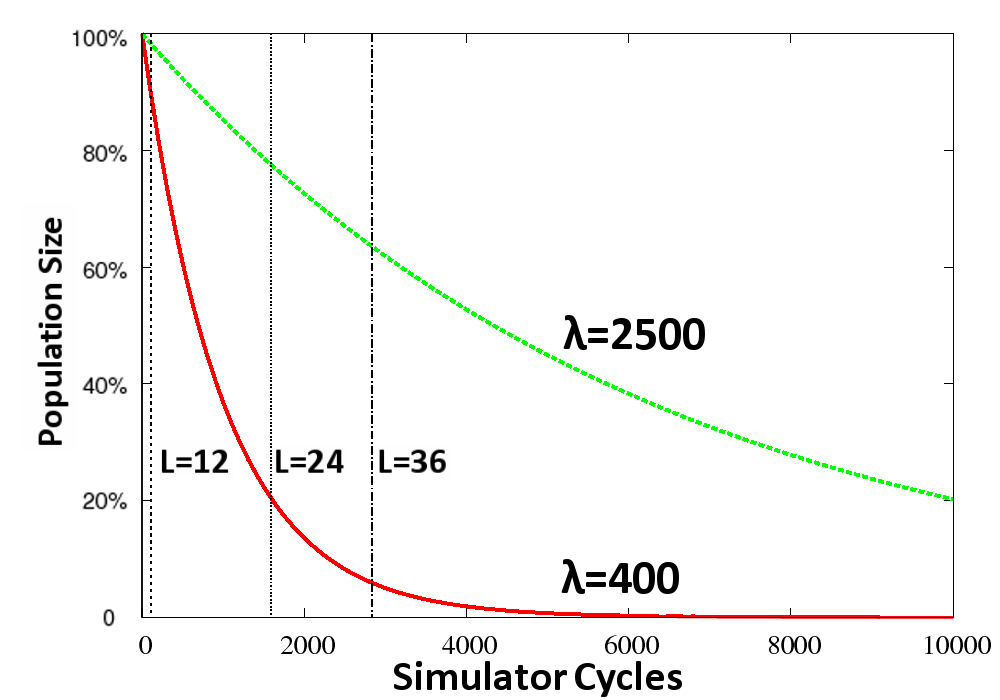
\includegraphics[width=0.7\textwidth]{failurerates}
\caption{Degradation of the system for the different failure rates and execution times in three instances of the 4-trap function.}
\label{fig:degradation}
\end{figure*}
%%%%%%%%%%%%%%%%%%%%%%%%%%%%%%%



\subsection{Analysis of the algorithmic convergence}
%%%%%%%%%%%%%%%%%%%%%%%%%%%%%%%%%%%%%%%%%%%%%%%%%%%%%%%%

This section analyses the convergence of the \evag approach in 2, 3 and 4-trap instances for different degradation rates $\lambda=400, 2500$ with respect to a failure-free execution. All settings are summarised in Table \ref{table:testcase3sca_secondserie}. 

Initial population sizes have been set to those values obtained in the previous series for the failure-free run of the selectorecombinative \evagp Using such values means that populations will be oversized for the failure-free counterpart in these series that use mutation. Nevertheless, that might not be the case when the system degrades. As previously seen, a small increase on the initial population size is sufficient condition for tolerating faults. Given that populations are oversized for a failure-free run using mutation, values will approximate an optimal size whenever the system degrades.




%%%%%%%%%%%%%%%%%%%%%%%%%%%%%%%%%%%%%%%%%%%%%%%%%%%%%%%%
\begin{table}[htbp]
\centering
{\scriptsize
\begin{tabular}{r l}
\multicolumn{2}{l}{\textbf{Trap instances}}\\
\hline
2-Trap & \\
Individual Length ($L$) & $60$\\
Population size & 135\\
Termination Condition & Max. Eval. = 5535\\
3-Trap & \\
Individual Length ($L$) & $60$\\
Population size & 480\\
Termination Condition & Max. Eval. =49920\\
4-Trap & \\
Individual Length ($L$) & $36$\\
Population size & 600\\
Termination Condition & Max. Eval. =393000 \\
&\\
\multicolumn{2}{l}{\textbf{GA settings}}\\
\hline
GA & \evag \\
Selection of Parents & Binary Tournament\\
Recombination & Uniform crossover, $p_c = 1.0$ \\
Mutation & Bit-flip mutation, $p_m = \frac{1}{L}$\\
&\\
\multicolumn{2}{l}{\textbf{Newscast settings}}\\
\hline
Cache size & 20\\
&\\
\multicolumn{2}{l}{\textbf{Scenarios of churn}}\\
\hline
$\lambda$ & 400,2500\\
$k$ & 0.4\\
\end{tabular}
}
\caption{Test-Case 3: Parameters of the experiments for the analysis of convergence.\label{table:testcase3sca_secondserie}}
\end{table}
%%%%%%%%%%%%%%%%%%%%%%%%%%%%%%%%%%%%%%%%%%%%%%%%%%%%%%%%


Figure \ref{fig:testcase3convergence} shows indeed that the \evag model converges better when the system degrades, specially in the worst case for $\lambda=400$. This fact is remarkable since the degradation of the system does not inflict a penalisation in the quality of solutions as could be expected but it is able to outperform the failure-free run despite \evags departing possibly contain valid solutions.

Besides, genetic diversity decreases faster as the system degradation turns more intensive which can be translated into a more exploitative behaviour of the algorithm. Such conclusion points out a possible explanation for the fault-tolerance of the model; as it has already been shown in Sections \ref{sec:testcase1} and \ref{sec:testcase2}, \evag is good at the preservation of genetic diversity and this way, it is able to balance the effect of an increasing exploitation component when the system degrades.

%%%%%%%%%%%%%%%%%%%%%%%%%%%%%%%
\begin{figure}[!htpb]
\centering
\subfigure{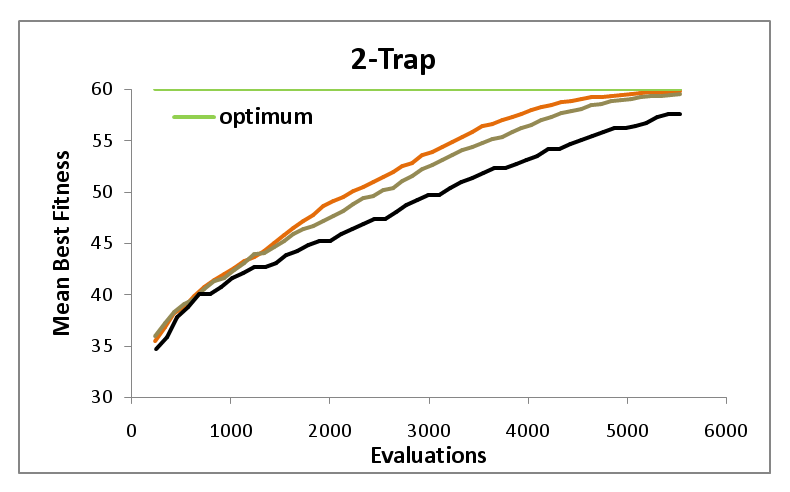
\includegraphics[width=2.9in]{churn2trapbestfitness}}
\hspace{1pt}
\subfigure{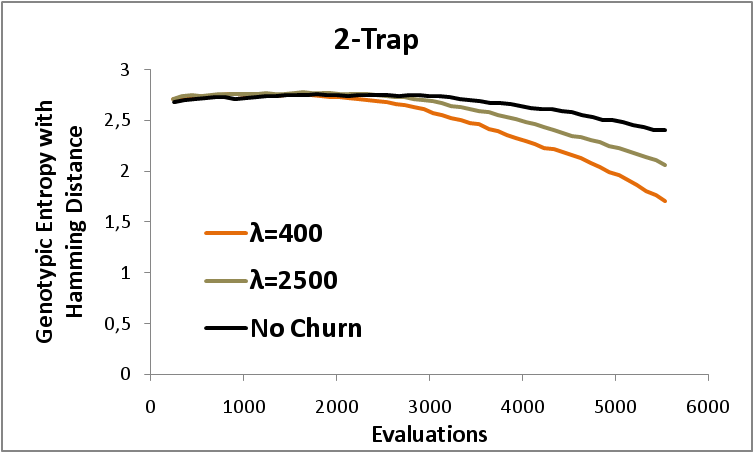
\includegraphics[width=2.9in]{churn2trapentropy}} \\
\subfigure{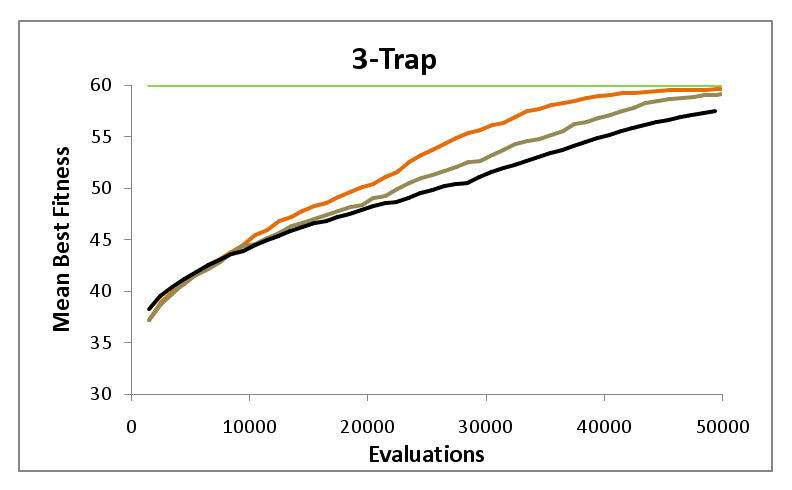
\includegraphics[width=2.9in]{churn3trapbestfitness}}
\hspace{1pt}
\subfigure{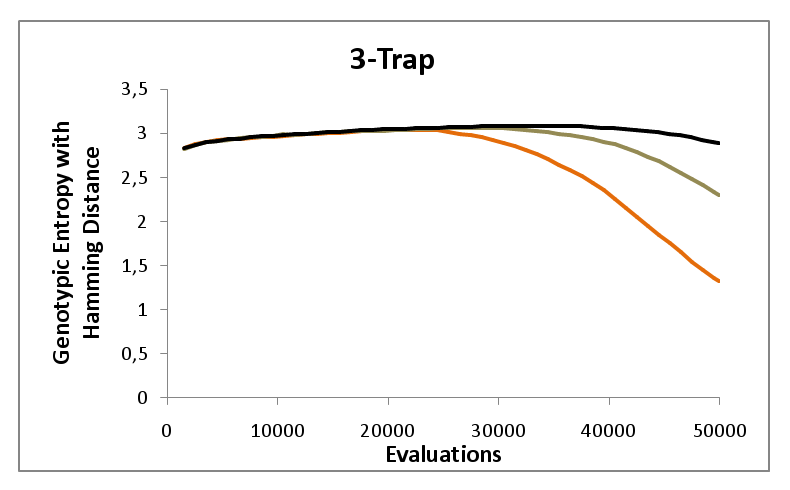
\includegraphics[width=2.9in]{churn3trapentropy}}\\
\subfigure{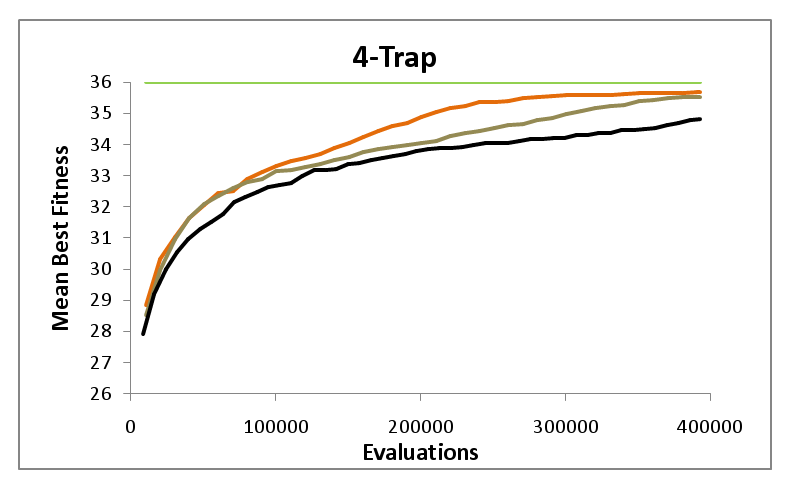
\includegraphics[width=2.9in]{churn4trapbestfitness}}
\hspace{1pt}
\subfigure{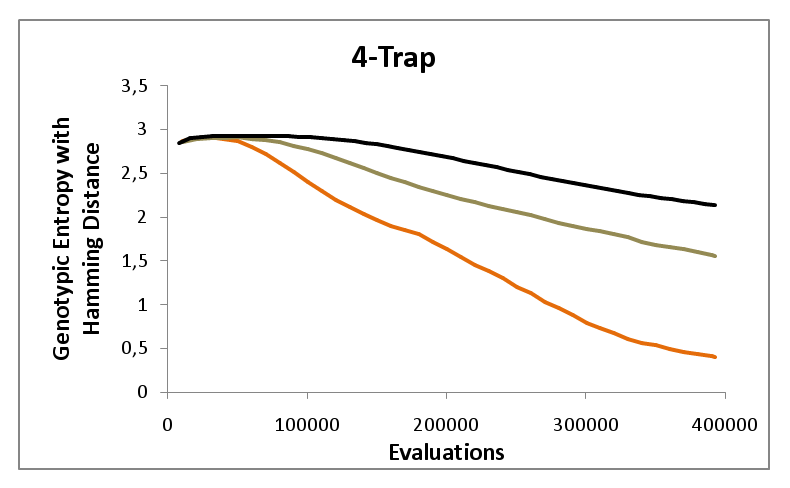
\includegraphics[width=2.9in]{churn4trapentropy}}
\caption{Test-case 3: Best fitness convergence ({\em left}) and evolution of the
  diversity expressed as the entropy based on the Hamming distances
  between the genotypes ({\em right}). Graphs plotted represent the
  average of 50 independent runs.}
\label{fig:testcase3convergence}
\end{figure}
%%%%%%%%%%%%%%%%%%%%%%%%%%%%%%%


Finally and providing a quantitative view on the run-time dynamics of {\em churn}, Figure \ref{fig:popdegradation} depicts the degradation of the population for the different runs in the 4-trap instance. It shows how the system degrades up to $\sim90\%$ in the worst case for $\lambda=400$.


%%%%%%%%%%%%%%%%%%%%%%%%%%%%%%%
\begin{figure*}[!htpb]
\centering
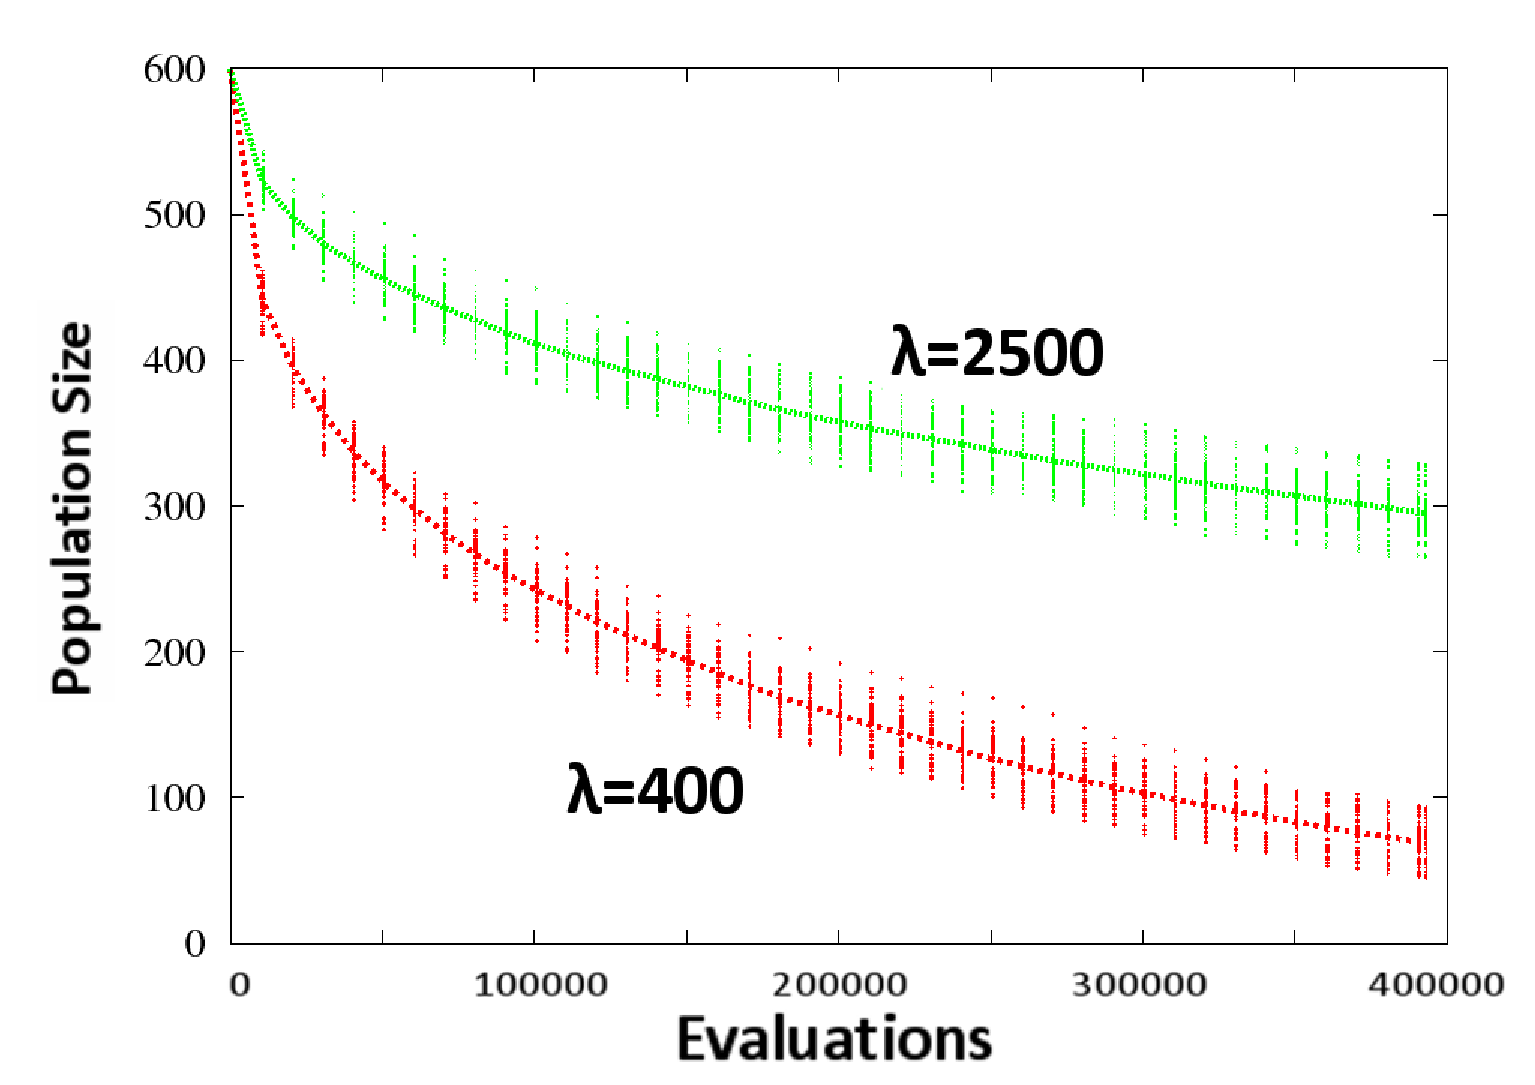
\includegraphics[width=0.7\textwidth]{popdegradation}
\caption{ Population dynamics in the 4-trap instance for $L=36$. Population sizes of the different runs are represented as points and the respective averaged values as lines for $\lambda=400$ and $\lambda=2500$.}
\label{fig:popdegradation}
\end{figure*}
%%%%%%%%%%%%%%%%%%%%%%%%%%%%%%%

\clearpage
\subsection{Statistical analysis}
%%%%%%%%%%%%%%%%%%%%%%%%%%%%%%%%%%%%%%%%%%%%%%%%%%%%%%%%

In order to provide previous results with an adequate statistical processing, Table \ref{table:comparativechurn} presents the Wilcoxon analysis of the data showing significant differences between the fitness distributions for the \evag model with and without failures in the system. 

The statistical analysis confirms the conclusion on the system degradation outperforming the failure-free run. In other words, the \evag model is inherently fault-tolerant and degrades gracefully.



%%%%%%%%%%%%%%%%%%%%%%%%%%%%%%%%%%%%%%%%%%%%%%%%%%%%%%%%%%%%%%
\begin{table*}[htbp]
\centering
{\tiny
\begin{tabular}{|c|c|c|c|c|}
\hline
{\it Problem Instance}&{\it Churn}&{\it Avg. Fitness $\pm\sigma$ }&{\it Wilcoxon Test }&{\it Significantly different?}\\
\hline
{\bf Trap2}	&				&			&	&\\
L=60		&$\lambda=400$	&{\bf	59.82$\pm$0.43	}&{\bf	W=184 p-value=6.32e-15	}&{\bf yes}\\
N=135		&$\lambda=2500$ &	59.5$\pm$0.78	&   W=320 p-value=2.9e-11	&yes\\
M. Eval.= 5535&{\it No Churn}&{\it 57.6$\pm$1.38}&-&-\\
\hline
{\bf Trap3}	&				&		& & \\
L=60		&{\bf $\lambda=400$	}&{\bf	59.62$\pm$0.62	}&{\bf W=414 p-value=1.37e-9 }&{\bf yes}\\
N=480		&$\lambda=2500$ &	59.14$\pm$1.2	&W=614 p-value=6.2e-6 &yes\\
M. Eval.= 49920&{\it No Churn}&{\it 57.5$\pm$2.04}&-&-\\
\hline

{\it Trap4}	&				&		& 	&\\
L=36		&{\bf $\lambda=400$	}& {\bf 35.68$\pm$0.46 }&{\bf W=447 p-value=1.89e-9 }& {\bf yes}\\
N=600		&$\lambda=2500$ &  35.54$\pm$0.69 & W=593 p-value=1.2e-6 & yes\\
M. Eval.= 393000&{\it No Churn}&{\it 34.82$\pm$0.66}&-&-\\

\hline
\end{tabular}
}
\caption{Wilcoxon test comparing the best fitness distribution of the \evag model under different {\em degradation} rates. Results are obtained over 50 independent runs.\label{table:comparativechurn}}
\end{table*}
%%%%%%%%%%%%%%%%%%%%%%%%%%%%%%%%%%%%%%%%%%%%%%%%%%%%%%%%%%%%%%


%%%%%%%%%%%%%%%%%%%%%%%%%%%%%%%%%%%%%%%%%%%%%%%%%%%%%%%%%%%%%
\subsection{Summary}

%%%%%%%%%%%%%%%%%%%%%%%%%%%%%%%%%%%%%%%%%%%%%%%%%%%%%%%%%%%%%

In this test-case, we have analysed the fault tolerance of the \evag model when running on a computing platform that degrades following the modelling of the churn dynamics established by Stutzbach and Rejaie in \cite{Stutzbach06Understanding}. To that aim, experiments were conducted on several instances of 2, 3 and 4-trap functions for different degradation rates. 

Through the experimental results we can conclude that {\em churn} does not damage the scalability order of the algorithm and a small increase on the initial population size is enough to keep a reliable convergence towards optimal solutions. In that sense, large instances of trap functions have been tackled with success  in spite of aggressive \emph{churn} conditions in which peers depart from the system until $90\%$ of the initial configuration is left.

In addition, the approach shows to be resilient to \emph{churn} with respect to execution time; once that the estimated population size guarantees a reliable convergence to the problem optimum, the
departure of nodes does not inflict a penalisation on the computational effort.

Therefore, the \evag model is fault-tolerant and implements a {\em graceful degradation} without any other extra mechanism than the emergent behaviour of the approach itself.

\clearpage


%%%%%%%%%%%%%%%%%%%%%%%%%%%%%%%%%%%%%%%%%%%%%%%%%%%%%%%%%%%%%
\section{Conclusions}
\label{sec:cap5:conclusions}
%%%%%%%%%%%%%%%%%%%%%%%%%%%%%%%%%%%%%%%%%%%%%%%%%%%%%%%%%%%%%



In this chapter, we have carried out an experimental analysis on the performance of the \evag model. To that aim, we investigate  the scalability and fault-tolerance of the approach in a simulated P2P environment. Such goals have been tackled in three different test-cases in which experiments are conducted on trap functions in order to assess the scalability of population sizes and computational efforts with increasing problem size and difficulty. 


In the first test-case, the scalability of the P2P model has been shown to outperform canonical panmictic approaches either in the population size or the computational efforts required to tackle the different problem instances. Furthermore, the improvement is specially outstanding as the problem difficulty increases pointing out that the \evag model is suitable for tackling large instances of difficult problems.

In the second test-case, we have analysed the influence of different population structures on the scalability of the approach. In that context, the choice of newscast as population structure has a positive effect on the algorithmic performance showing better times to solution than the ring lattice in every problem instance and equivalent performances to the Watts-Strogatz approach. 


Finally, the third test-case focuses on the fault-tolerance of the model when running on failure prone platforms that degrade following two different churn rates. Results show that a small increase on the initial population size is a sufficient mechanism to guarantee the convergence of the approach, in turn, such an increase does not inflict a penalisation on the computational effort.


This way and going back to the goals pose at the beginning, it can be concluded that the \evag model is scalable and fault-tolerant.



%\bibliographystyle{alpha}  % Eliminarlo al compilar el documento maestro, ponerlo para compilarlo separado
%\bibliography{evagperformance,pea,p2pcomputing,model,methodology} %Eliminarlo al compilar el documento maestro, ponerlo para compilarlo separado

%\end{document}             % Eliminarlo al compilar el documento maestro, ponerlo para compilarlo separado
